\chapter{Evaluation}
\label{cha:evaluation}

In this chapter we will delve into the results from the several trainings we performed with the agents. We will deeply explain the results and discuss them to try to extract insightful knowledge from it. First we will discuss the several models, and computers we have used along this work. We will also compare the models in term of computational complexity, giving a deeper sight on the training times considered in this work. Finally we will go over the explainability results that we have obtained, and discuss if they are insightful in terms of understanding whether the attention-models explain their own behaviour with the attention maps and the explainability techniques already discussed.

\section{Experimental set-up}
\label{sec:exp_setup}

\subsection{Computing resources}
To carry out our experiments, we used several computers with several GPUs to meet the time constrains that this work imposed. According to several works \cite{mnih2013playing, hessel2017rainbow, schaul2016prioritized, meng2024deep}, the usual number of training steps for DQN learning algorithms is between 50 million and 200 million steps. We could not achieve this for any of our training procedures. Even though the GPUs we used for our training were powerful, they cannot compare to the resources that companies such as Google DeepMind has. For the development of this work, we used 4 different computers:

\begin{enumerate}
	\item Computer 1 - Personal computer with the following specs:
	\begin{itemize}
		\item CPU: AMD Ryzen 5600X.
		\item GPU: 1 $\times$ NVIDIA RTX 3060 (12 GB of GDDR6 VRAM).
		\item RAM: 32 GB of DDR4.
	\end{itemize}
	\item Computer 2 - Universidad de Alcalá with the following specs:
	\begin{itemize}
		\item CPU: AMD Ryzen 9 5950X.
		\item GPU: 2 $\times$ NVIDIA RTX 3080 (10 GB of GDDR6X VRAM).
		\item RAM: 32 GB of DDR4.
	\end{itemize} 
	\item Computer 3 - Artemisa cluster (Universidad de Valencia and Universidad de Alcalá) with the following specs (we only specify the resources we were allowed to use):
	\begin{itemize}
		\item CPU: Intel(R) Xeon(R) Gold 6130 CPU @ 2.10GHz
		\item GPU: 1 $\times$ NVIDIA V100 (40GB of HBM2e)
		\item RAM: 32 GB of DDR4
	\end{itemize} 
	\item Computer 4 - Anomalia cluster (Universidad Autónoma de Madrid) with the following specs (we only specify the resources we were allowed to use):
	\begin{itemize}
		\item CPU: Intel(R) Xeon(R) Silver 4210R CPU @ 2.40GHz.
		\item GPU: 3 $\times$ NVIDIA RTX 3090 (24 GB of GDDR6X VRAM).
		\item RAM: 196 GB of DDR4.
	\end{itemize} 
\end{enumerate}

The use of this systems made possible to accelerate the training speeds, but we could not get their full potential such as training parallelization. We tried to implement a training procedure similar to \cite{stooke2019rlpyt} where they implement a library to accelerate inference times and sampling from the experience replay buffer across GPUs using MPI \cite{gropp_using_1994} in python using PyTorch. We tried to do something similar in our implementation, but could not make it to work.

\subsection{Training set-up}
For the training procedure, we run the models under just one constrain: to end the training if for a portion of the total trained steps until that time, no improvement is done. We were aware that for a lot of training set-ups, the model may face a streak where does not improve for a long period of time, and then, out of the blue, starts to pick up knowledge and exploits it obtaining great scores down the line. We could not afford to do this, given our time constrains, and "limited" resources. Referring to the hyper-parameters used in the training procedures, we fixed the ones that were related to the agent training, such as the $\gamma$, the learning rate, the batch size or the initial and final exploration rates (see Table \ref{tab:hyper-parameters}). We have seen that in several works, such as \cite{vanhasselt2015deep, hessel2017rainbow, meng2024deep}, they implement the same thing for the training procedure.

\begin{table}[!h]
	\begin{center}
		\caption[Fixed hyper-parameters that are shared across different training procedures.]{Fixed hyper-parameters across different training procedures.}
		\label{tab:hyper-parameters}
		\begin{tabular}{||c | c||} 
			\hline
			Input & 84 $\times$ 84 $\times$ 4 \\
			\hline
			Optimizer & Adam \\
			\hline
			Adam Learning Rate & $6.25 \times 10^{-5}$ \\
			\hline
			$\gamma$ & 0.99 \\
			\hline
			Initial $\epsilon$ & 1 \\
			\hline
			Final $\epsilon$ & 0.01 \\
			\hline
			$\epsilon$-decay steps (frames) & 1 $\times 10^6$   \\
			\hline
			SyncFrames & $4 \times 10^4$ \\
			\hline
			SkipLearningFrames & 4 \\
			\hline
			Replay Buffer Size & $1 \times 10^{6}$ \\
			\hline
			Batch Size & 32 \\
			\hline
		\end{tabular}
	\end{center}
\end{table}

\subsection{Q-networks configuration}

For each of the Q-networks, the hyper-parameters related to the topology of the networks varies in terms of layers, and the number of weights. Additionally, we also trained a series of models using a CNN similar to the one used in \cite{vanhasselt2015deep} to obtain a "baseline" on the performance and perform different experiments in the exploration schedules, since their computational complexity is inferior to the attention-based models, and given the results, we selected the exploration schedule accordingly.

The hyper-parameters related to the models are defined in tables \ref{tab:vit-small-hyper-parameters}, \ref{tab:vit-big-hyper-parameters} and \ref{tab:swin-hyper-parameters}. In the case of the SWIN DDQN network, we copied the same topology as the one proposed in \cite{meng2024deep}. In the case of the ViT DDQN network, we tried to balance between the number of weights from the model and the computation complexity of the forward and backward pass, given the quadratic computational complexity from the model. We designed two configurations: ViT-Big and Vit-Small, but because of time constrains, we only could train the ViT-Small configuration.

Additionally, since to the best of our knowledge, we have not seen any work that explores the ViT as the backbone for a value function approximation in DQN-learning, and for the SWIN Transformer, we have stated that there are some works that explore this set-up, but no pre-trained weights where available, which meant we did not have a baseline to start from when training the agents.

\begin{table}[!h]
	\begin{center}
		\caption[CNN DDQN network hyper-parameters]{CNN DDQN network hyper-parameters}
		\label{tab:cnn-hyper-parameters}
		\begin{tabular}{||c | c||} 
			\hline
			Layers & 3 \\
			\hline
			Filters per layer & 32, 64, 64 \\
			\hline
			Number of heads per block & 6 \\
			\hline
			Linear dimension after flatten & 512 \\
			\hline
			Activation function & ReLU \\
			\hline
		\end{tabular}
	\end{center}
\end{table}

\begin{table}[!h]
	\begin{center}
		\caption[ViT Small DDQN network hyper-parameters]{ViT Small DDQN network hyper-parameters}
		\label{tab:vit-small-hyper-parameters}
		\begin{tabular}{||c | c||} 
			\hline
			 Layers & 5 \\
			 \hline
			 Blocks per layer & 1 \\
			 \hline
			 Number of heads per block & 6 \\
			 \hline
			 Embedding dimension & 156 \\
			 \hline
			 Patch size & 7 \\
			 \hline
			 Dropout rate & 0.1 \\
			 \hline
		\end{tabular}
	\end{center}
\end{table}

\begin{table}[!h]
	\begin{center}
		\caption[ViT Big DDQN network hyper-parameters]{ViT Big DDQN network hyper-parameters}
		\label{tab:vit-big-hyper-parameters}
		\begin{tabular}{||c | c||} 
			\hline
			Layers & 5 \\  
			\hline
			Blocks per layer & 1 \\
			\hline
			Number of heads per block & 8 \\
			\hline
			Embedding dimension & 208 \\
			\hline
			Patch size & 5 \\
			\hline
			Dropout rate & 0.1 \\
			\hline
		\end{tabular}
	\end{center}
\end{table}

\begin{table}[!h]
	\begin{center}
		\caption[SWIN DDQN network hyper-parameters]{SWIN DDQN network hyper-parameters}
		\label{tab:swin-hyper-parameters}
		\begin{tabular}{||c | c||} 
			\hline
			Layers/Stages & 3 \\ 
			\hline
			Blocks per layer & 2,3,2 \\
			\hline
			Heads per layer & 3,3,6 \\
			\hline
			Patch Size & 3 $\times$ 3 \\
			\hline
			Window Size & 7 $\times$ 7 \\
			\hline
			Embedding dimension & 96 \\
			\hline
			Dropout rate & 0.2 \\
			\hline
		\end{tabular}
	\end{center}
\end{table}

Additionally, we state in Table \ref{tab:models_parameters} the number of weights each backbone that we trained our agent on had. We used the \inlinecode{torchinfo} \cite{torchinfo} library to obtain these estimations. We state the floating operations per second (FLOPs) for the proposed models using the \inlinecode{ptflops} library \cite{ptflops}. The code where we compute the values is available in scripts \href{https://github.com/Javimh18/DL_TFM/blob/main/src/models/size_calculator.py}{size\_calculator.py} and \href{https://github.com/Javimh18/DL_TFM/blob/main/src/models/flops_calculator.py}{flops\_calculator.py}. It is clear that the CNN is the model with less computational complexity, since it has far less FLOPs than the rest of the networks. For the ViT-Small we see that the complexity increases significantly with respect to the number of parameters, as it has roughly the same of parameters as the CNN, but far more FLOPs due to the attention mechanism. The SWIN transformer is by far the most complex model in terms of parameters, with almost 3 times the number of parameters from the ViT-Small and CNN, and almost 72 times more computational complexity in terms of FLOPs than the CNN. Additionally, the ViT-Big model has only 1.5 more parameters than the CNN, but more FLOPS than the SWIN Transformer (almost 75 times more). With this comparison we try to reflect the great computational cost that comes with the attention-based models in the deep learning paradigm.

\begin{table}[h!]
	\begin{center}
		\caption[SWIN DDQN network hyper-parameters]{Number of parameters and FLOPs per model per forward pass.(Note: We put the scales in orders of megas and gigas (i.e. $10^6 \text{, } 10^9$) for a better understanding of the units)}
		\label{tab:models_parameters}
		\begin{tabular}{|c|c|c|c|}
			\hline
			Q-network & Number of Parameters & MACs & FLOPs \\  [0.5ex] 
			\hline
			\hline
			CNN & 1.69 $\times 10^6$ & $9.41 \times 10^6$ & $18.42 \times 10^6$ \\ 
			\hline
			VIT Small & 1.52 $\times 10^6$ & $218.07 \times 10^6$ & $436.14 \times 10^6$ \\ 
			\hline
			VIT Big & 2.68 $\times 10^6$ & $677.05 \times 10^6$ & $1.354 \times 10^9$ \\ 
			\hline
			SWIN & 5.49 $\times 10^6$ & $644.92 \times 10^6$ & $1.289 \times 10^9$ \\ 
			\hline
		\end{tabular}
	\end{center}
\end{table}

\subsection{Environments}

Pac-man is an widely known video-game launched for the Atari 2600 console back in the eighties. In the game, we take part as Pac-Man, a pie-shaped creature that moves around a maze. The main goal of the game is to stay alive by eating the dotted rewards, called \textbf{tiles} around the maze while avoiding the coloured ghosts:  Blinky, Pinky, Inky, and Clyde. Scattered throughout the maze, there are a set of rectangles that have the power of turning the coloured ghosts to blue for a short period amount of time. When this happens, Pac-Man can eat the ghosts, and win additional points. When we eat all the dots from the maze, we level-up, to more complex mazes when we have to repeat this process. The player is limited to 8 moves: UP, DOWN, LEFT, RIGHT, UP-LEFT, UP-RIGHT, DOWN-LEFT and DOWN-RIGHT. In Figure \ref{fig:pacman} we show a screenshot of the game.

Demon Attack is also a Atari game where players battle against the enemies in the form of demons. Each wave of demons presents a new challenge, growing more difficult and aggressive as the game progresses. Some of these alien adversaries even split into smaller demons when struck, adding an extra layer of complexity to the gameplay. The game’s controls are simple: SHOOT, LEFT, RIGHT. The main goal is to survive while shooting and killing the demons to obtain higher rewards. In Figure \ref{fig:demon_attack} we show a screenshot of the game.


\begin{figure}[!h] 
	\centering
	\subfloat[MsPacman environment.]{%
		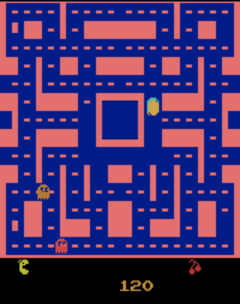
\includegraphics[width=0.45\linewidth]{figures/pacman.png}%
		\label{fig:pacman}%
	}%
	\hfill%
	\subfloat[Demon Attack environment.]{%
		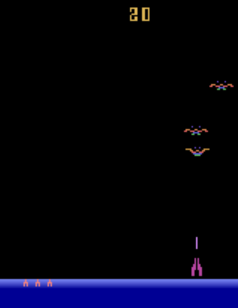
\includegraphics[width=0.45\linewidth]{figures/demon_attack.png}%
		\label{fig:demon_attack}%
	}%
	\caption{In figure \ref{fig:pacman} (left) we see the Pacman environment. In figure \ref{fig:demon_attack} (right) we see the Demon Attack environment.}
	\label{fig:envs_to_test}
\end{figure}

\section{Training results}
\label{sec:env_setup}

\subsection{Exploration schedules}
\label{sec:eval_exp_schedules}

In section \ref{sec:schedulers} we introduced three different types of scheduling: exponential decay, linear decay and product of exponents decay. To know which schedule we had to use for our final training procedures, we had to test them out. To do so, we used the CNN models as our test model for trying the different schedules. This decision was taken mainly because of time constrains, as we have seen in Table  \ref{tab:models_parameters} that CNNs are the less computational expensive model. We trained all the models in the computer 2 (mentioned in section \ref{sec:exp_setup}) for $1.2 \times 10^7$ steps using the DDQN algorithm and checked which one got better results according to the experimental set-up defined in Table \ref{tab:hyper-parameters}. The environment where we made these tests was \textbf{MsPacman-v5}. We are aware that this may not be the best way to test these results, but given the amount of time that we had at our disposal, it was the only plausible way to test different schedules and take a decision on which one was better for our final results. The comparison of the evolution can be seen in Figure \ref{fig:comp_cnn_schedulers}.

\begin{figure}[!h]
	\centering
	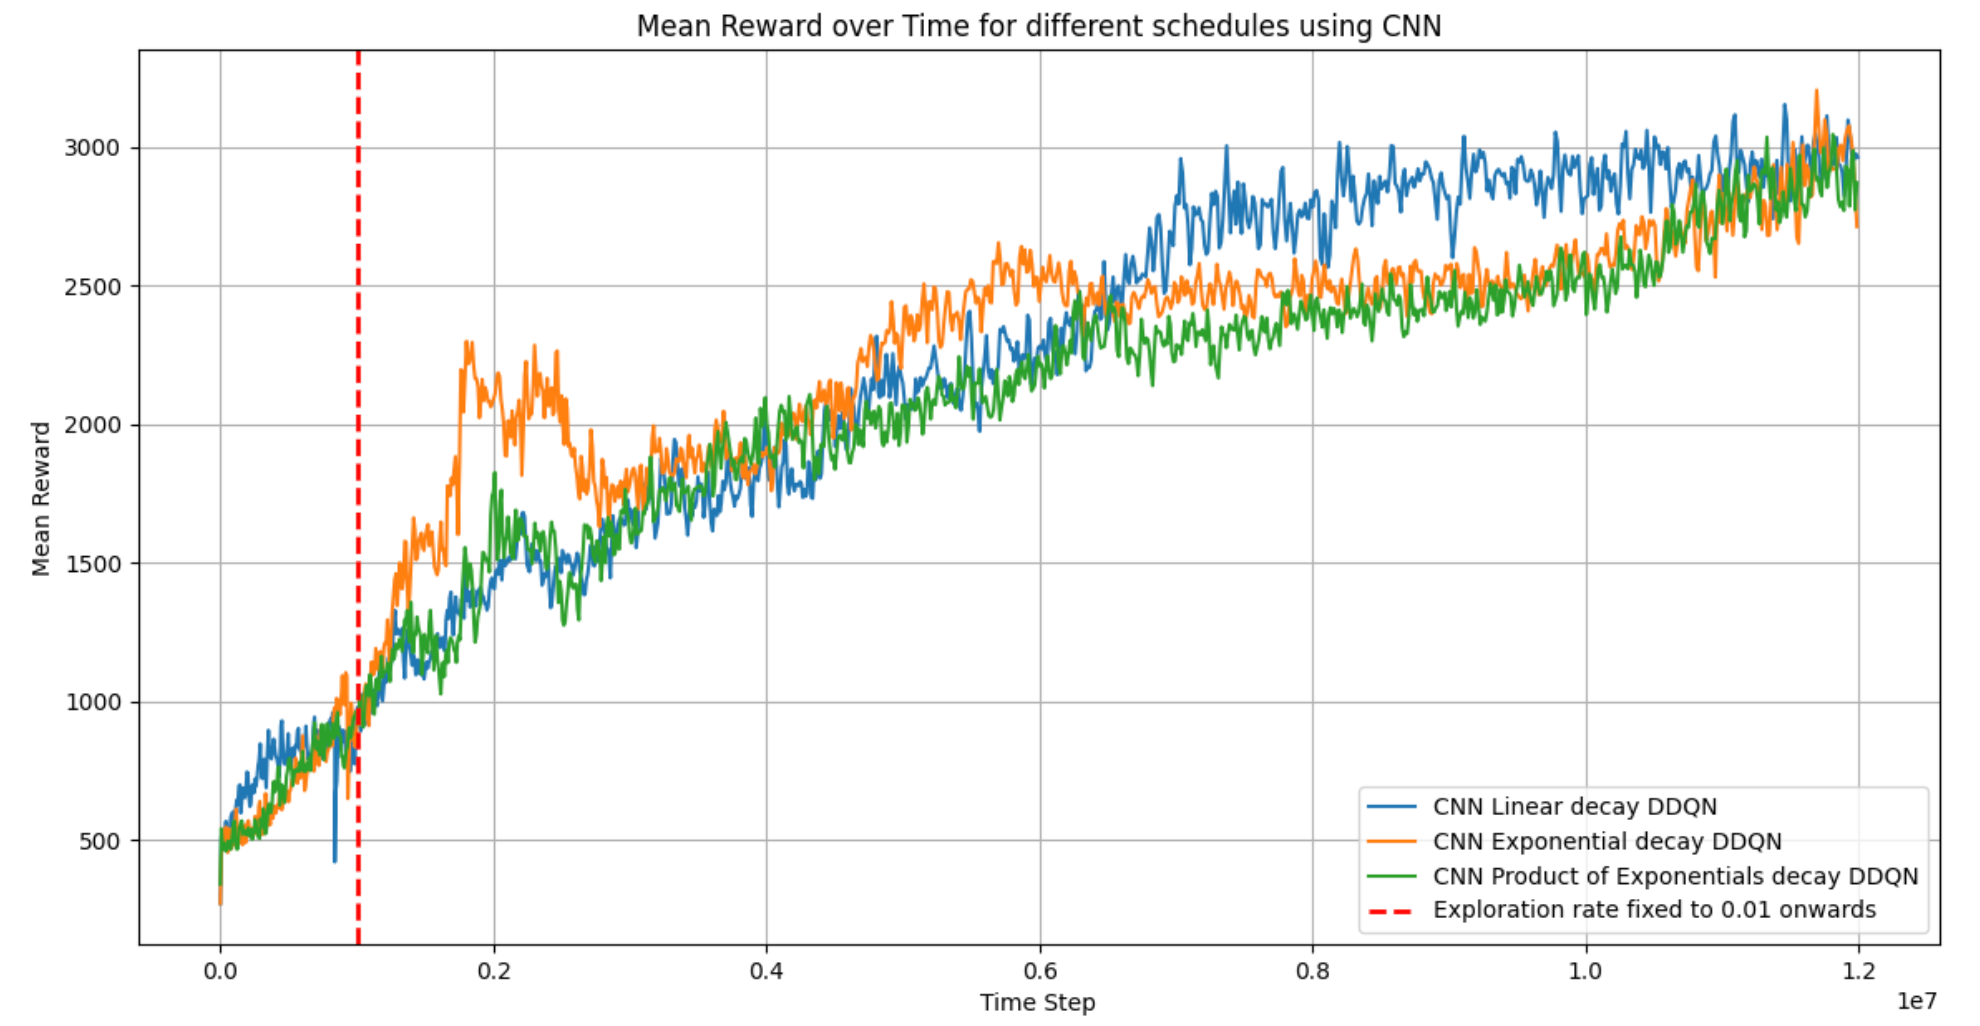
\includegraphics[width=\linewidth]{figures/comp_sch_12M}
	\caption{Comparison between different schedules for a DDQN CNN agent for $1.2 \times10^7$ steps.}
	\label{fig:comp_cnn_schedulers}
\end{figure}

We can see that the there is no better performing schedule up until that point. For us, this was it bit strange, since we expected that the linear and power of exponentials schedules would come up top, since the had higher exploration rate for a longer time than the exponential schedule. It was in this point where we decided to opt for the product of exponentials for the rest of the training procedures, since up until the 12 million steps mark, it was the schedule with the greater growth in the last 6 million steps, even if it was marginal. The training time to reach for the 12 million steps mark was around 1 days and 12 hours each approximately. We kept training the agents with these three different schedules and, after almost 3 days and 20 hours of training we found a counter-intuitive surprise in the 25 million steps mark, as can be seen in Figure \ref{fig:compsch25m}, where the exponential decay was actually the best performing schedule from all of them. We say "counter-intuitive" because we held onto the intuition that since the linear schedule and the product of exponentials had more exploration rate for a bigger amount of time, it would help the agent to collect a wider variability of experiences and perform better estimations. If we would have more time to test the proposed schedules, trying different runs and testing which schedule came up on top more consistently, maybe we could have taken a more insightful decision on which schedule select.

\begin{figure}[!h]
	\centering
	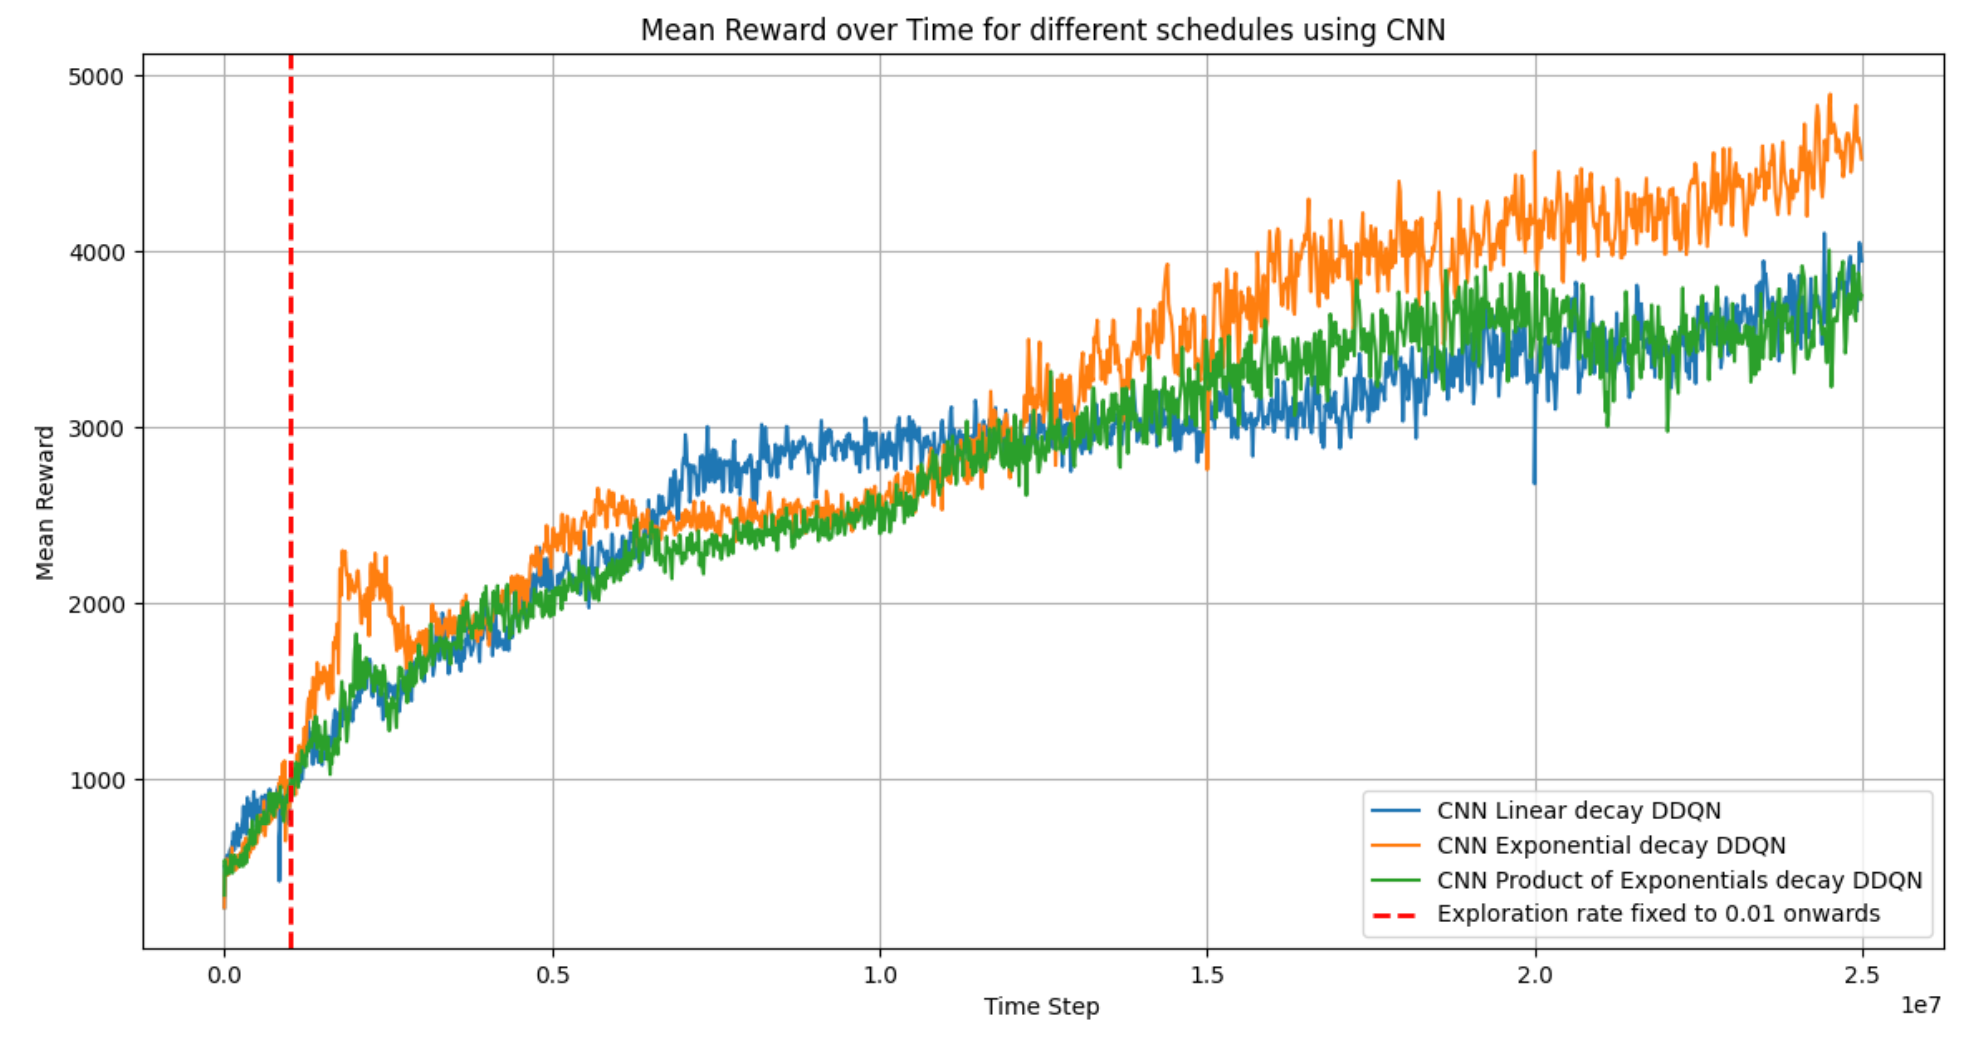
\includegraphics[width=\linewidth]{figures/comp_sch_25M}
	\caption{Comparison between different schedules for a DDQN CNN agent for $2.5 \times10^7$ steps.}
	\label{fig:compsch25m}
\end{figure}

\subsection{Agents training comparison}
\label{sec:eval_comp_models}
As stated in section \ref{sec:eval_exp_schedules}, in the 12 million mark from the comparison training, we selected the product of exponentials as our exploration schedule for \textbf{all} the training procedures. We were on a hurry to launch all of our experiments for both MsPacman-v5 and DemonAttack-v5 environments, since we knew the computational cost the proposed Q-networks had. We selected to train our agents in two different environments to compare how the explainability mechanisms behaved in different environments, and if an interpretable set-up was achieved in both of them. In the following sections we will briefly introduce the rules of the games and show the obtained results in both training and evaluation phases.

\subsubsection{MsPacman training results}
\label{sec:mspacman-training-results}
For the this environment, we launched the three training procedures and let them train as much as we could. The training time for all of the models went over 6 days, and the training was run in Computer 4. The results are portrayed in Figure \ref{fig:pacmanfinalresults}. For the ViT agent, we trained a total of 4.5 $\times 10^7$ steps with a maximum reward of 5811. For the SWIN agent, we trained a total of 3 $\times 10^7$ steps with a maximum reward of 5637. For the CNN agent, we trained a total of 6 $\times 10 ^7$ steps, with a maximum reward of 5369. The red dashed line represents the point where the exploration schedule finished, remaining the exploration rate in a fixed value of $\epsilon$=0.01. 

\begin{figure}[!h]
	\centering
	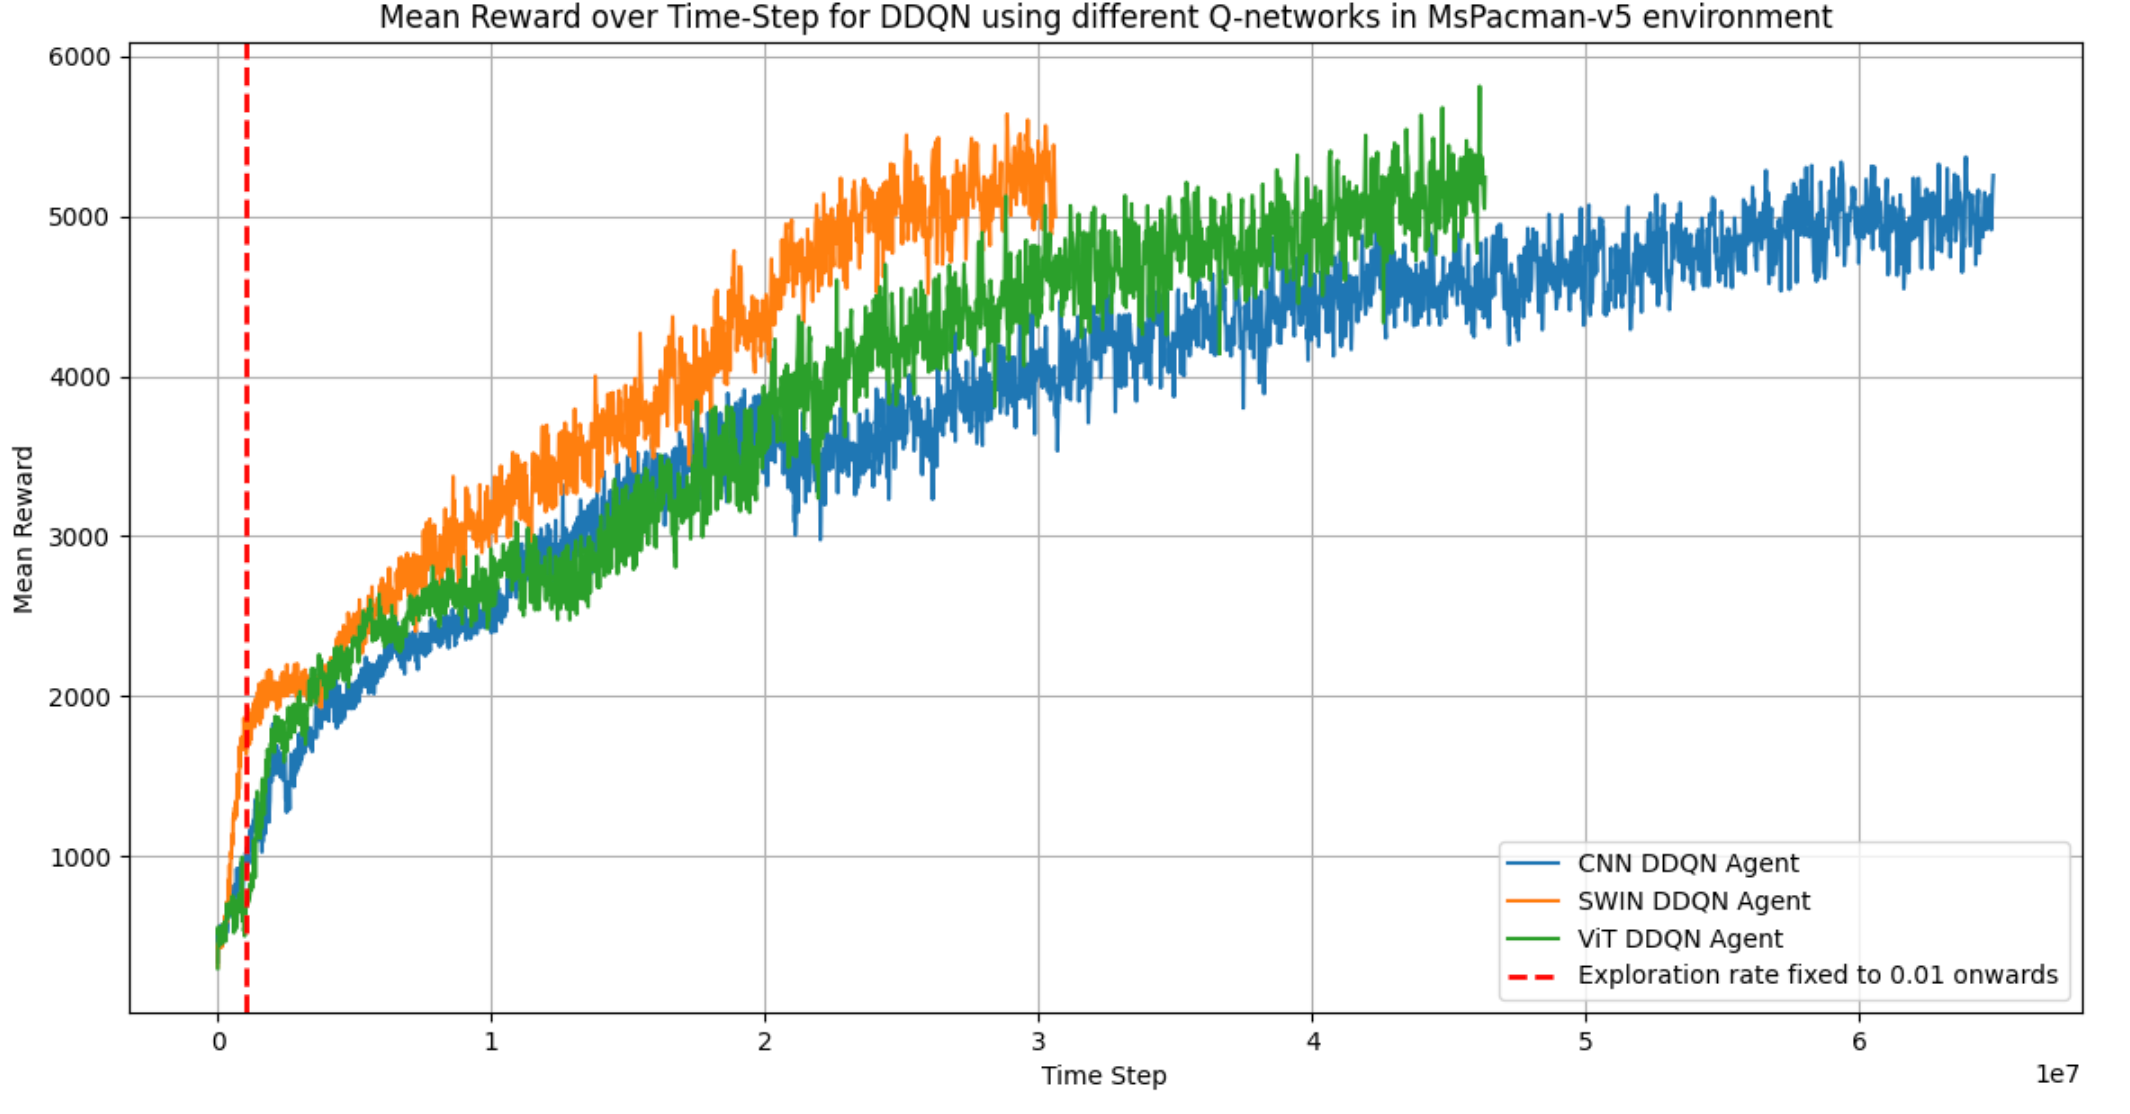
\includegraphics[width=0.9\linewidth]{figures/pacman_final_results}
	\caption{Reward vs. Time-steps for the CNN, SWIN and ViT agents.}
	\label{fig:pacmanfinalresults}
\end{figure}

It is pretty clear that the CNN agent was the one with more time-steps to train, with over 6.5 $\times 10^7$, given its lower computational complexity, allowing to play more episodes and explore more in the environment. The ViT agent was the one with more steps to train, with roughly over 4.5 $\times 10^7$. Finally, the SWIN agent was the one that got less steps of training, with a bit more of 3 $\times 10^7$. It is clear that the CNN agent is the model with less parameters, and the one that needs more time and experiences to actually learn, but it collects experiences faster which compensates, obtaining a competitive reward. The ViT transformer is actually the most efficient in terms of ratio between number of parameters per point of reward. It is also quite evident that even though having a bit less number of parameters compared to the CNN, it actually needs far less number of steps to converge to the same reward, leveraging of the attention mechanism to extract richer features that estimate better situations, probably giving better estimations for the Q-values. The SWIN transformer is clearly the most complex model, which justifies the faster learning in terms of time-steps, as its reward curve ascends faster than the rest in terms of time-steps. It is also the less efficient model in terms of number of parameters per point of reward. But overall, the phenomena that surprised us the most is the CNN being able to compete with the attention-based models, even though it is far more simpler. 

Additionally, we also display in Figure \ref{fig:pacmanfinalresultsinseconds}  a chart that compares the reward against the time in seconds. There, the red dashed line represents the point where the exploration schedule finished for the CNN model, the magenta dashed line does the same for the SWIN agent and the purple for the ViT agent. The remaining exploration rate for the training will remain in a fixed value of $\epsilon$=0.01. It is quite interesting how the CNN agent actually learns faster in time compared to its the attention-based counter-parts. We associate this to the lower complexity of the model, and having far less parameters, which actually benefits in terms of convergence for the weight's values. 

\begin{figure}[!h]
	\centering
	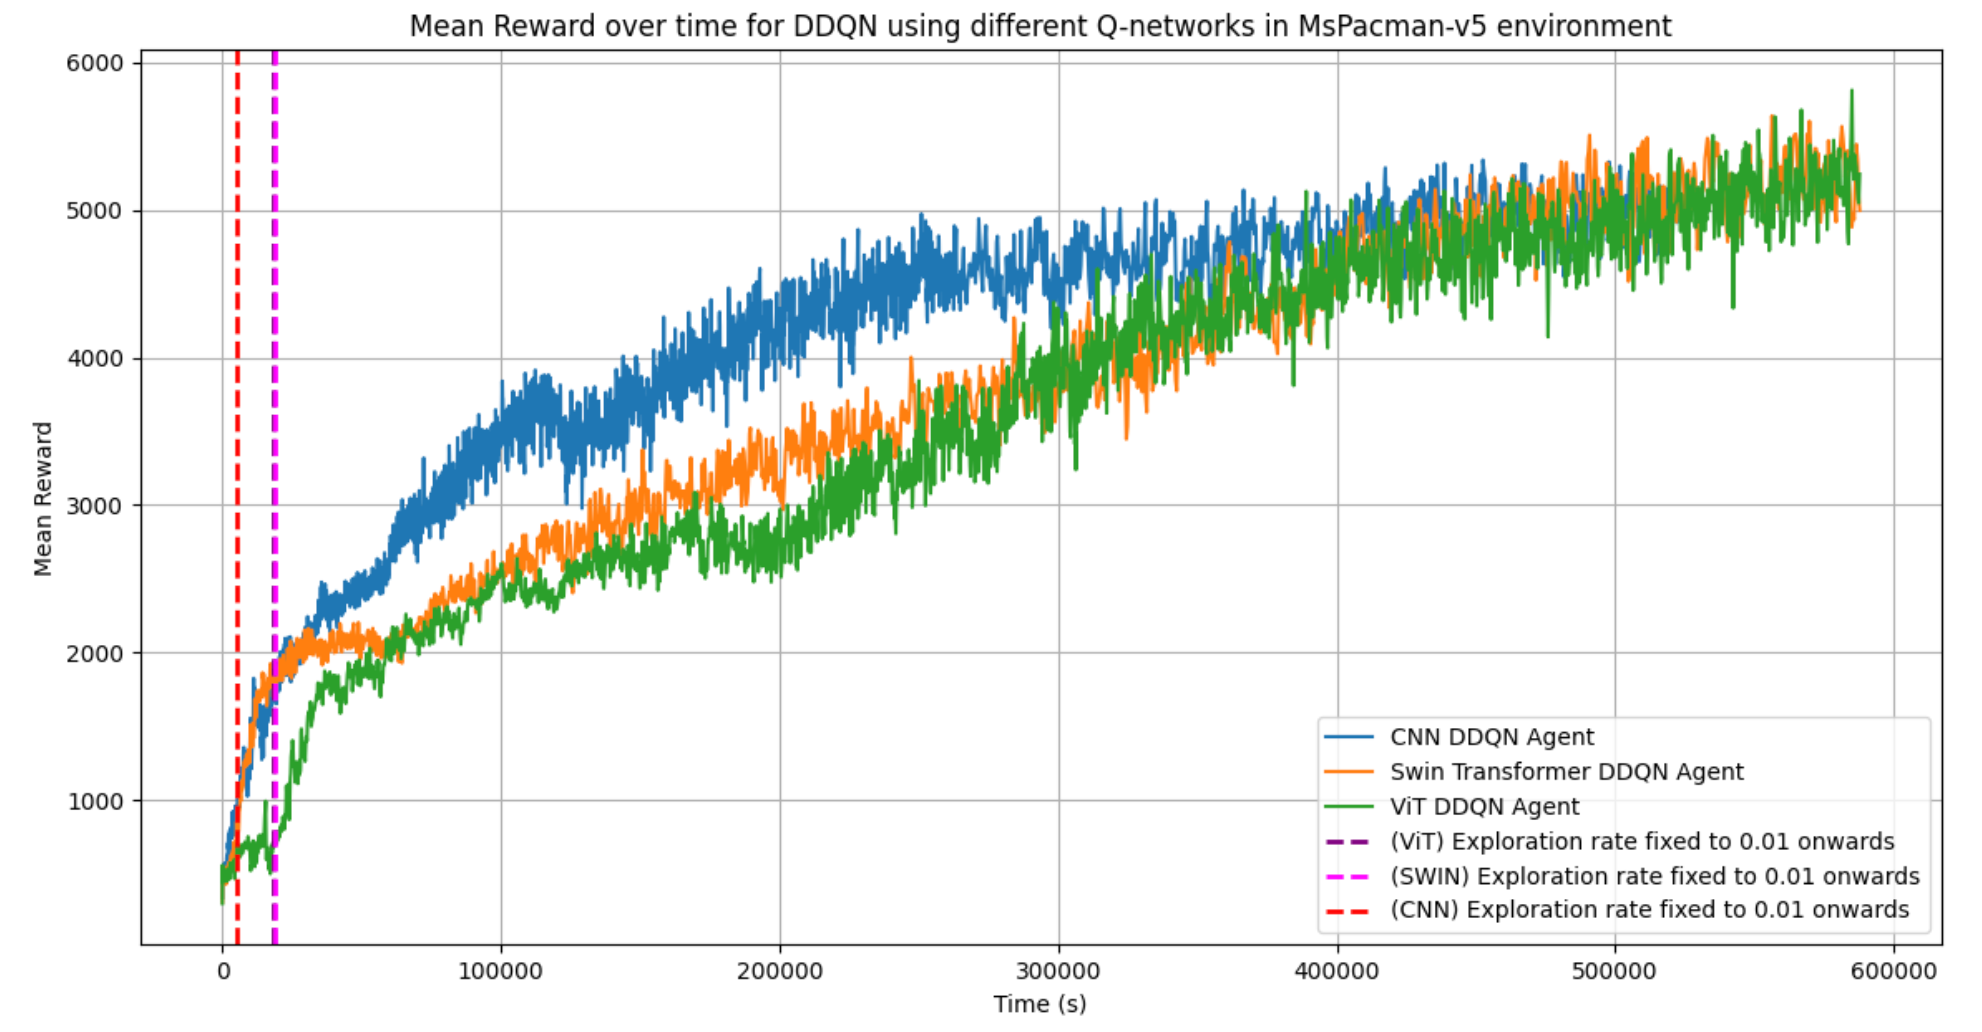
\includegraphics[width=\linewidth]{figures/pacman_final_results_in_seconds}
	\caption{Reward vs. Time in seconds for the agents in MsPacman environment.}
	\label{fig:pacmanfinalresultsinseconds}
\end{figure}

We can also see, even though is a bit overlapped that the CNN agent started to stuck around the second 2.5 $\times 10^5$ since the reward did not pick up for the rest of the training. This maybe because the CNN agent has a harder time improving as the game becomes more difficult, which is probably associated with its smaller amount of parameters. On the other hand, the attention-based models follow a similar pattern, by constantly improving, and achieving better results. It is clear that the attention-based models had potential to achieve higher rewards, and we wonder how they would have been if we could have the time to train them until no improvement was shown. As a final recap, in Table \ref{tab:pacman_trainingresults} we sum up the essential information.


\begin{table}[!h]
	\begin{center}
			\caption[MsPacman environment results for the several trained agents]{MsPacman environment results for the several trained agents}
			\label{tab:pacman_trainingresults}
			\begin{tabular}{||c c c c | c||} 
					\hline
					Agent type & Total Time (s) & Total Steps & Total Episodes & Max. Reward \\ [0.5ex] 
					\hline\hline
					CNN & 6 days 4 hours& 6.4881 $\times 10^7$ & 192000 & 5369 \\ 
					\hline
					SWIN & 6 days 19 hours & 3.0978 $\times 10^7$ &  93850 & 5637 \\
					\hline
					ViT & 6 days 19 hours & 4.6775 $\times 10^7$ &  145552 & \textbf{5811} \\
					\hline
				\end{tabular}
		\end{center}
\end{table}

\subsubsection{DemonAttack training results}
\label{sec:demon-attack-training-results}

For the DemonAttack environment, we followed a similar training approach as with the PacMan environment.  We launched the models and trained them as much as we could, but, in the moment we saw that the progress in the reward stalled, we killed the training procedure. The training procedures for the attention-based Q-network agents went over 7 days, while the CNN Q-network agent was only run for over 2 days. We will explain the reason of this later in this section. The final training procedures were run in Computer 2. In Figure \ref{fig:demonattackresultsts} we show the training results for our agents. 

\begin{figure}[!h]
	\centering
	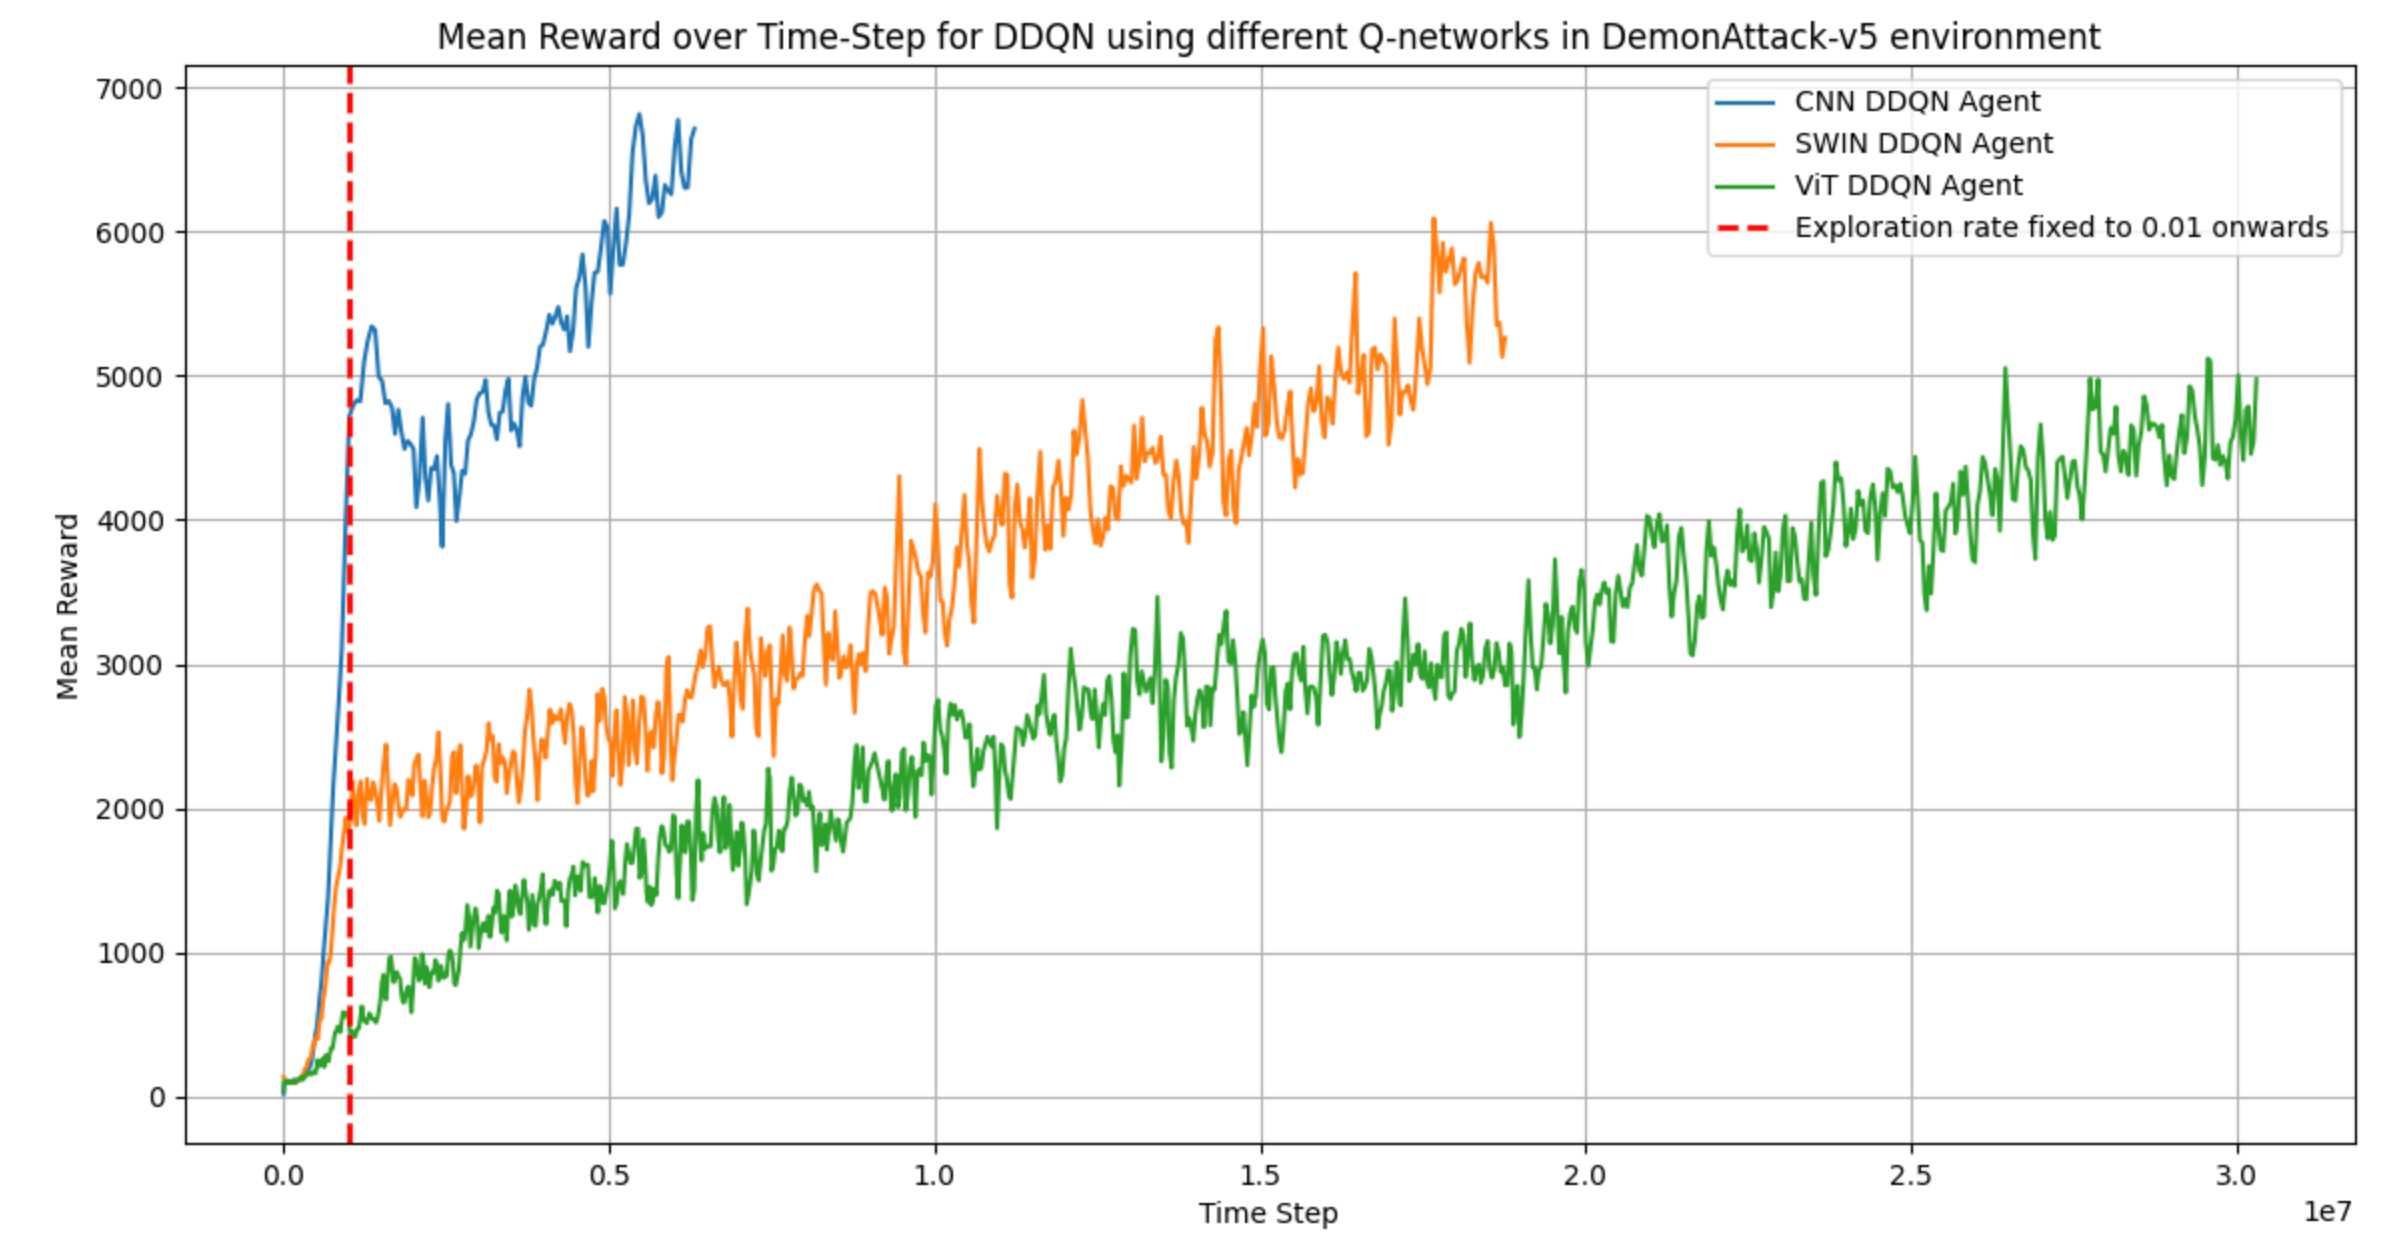
\includegraphics[width=\linewidth]{figures/demon_attack_results_ts}
	\caption{Demon Attack environment results in time-steps. }
	\label{fig:demonattackresultsts}
\end{figure}

The progress in the training steps remains constant for the attention-based agents, as they linearly improve obtaining more rewards over time. Given the results of the previous section, we opted to only train the attention-based agents, since they over-performed the CNN. As we launched the training, we face the situation where the learning was too slow. Just to give an idea, in \cite{meng2024deep} for just 50 million steps, the mean reward was around 80.000, while for our agents, after 30 million steps, it was just 4.000 for the ViT agent. Given these results, we launched the CNN agent to see if it was an issue with the set-up or with the Q-networks of our agents. 

It was pretty clear that, as we launched the CNN agent, it started to score far better results than the attention-based agents. We do not have an explanation for this, since we did not expected these results, specially with short amount of time that we train it. It caught our eye how just in the exploration period, the CNN completely outperforms the ViT and the SWIN agent by large amounts of reward. Additionally, the difference between the ViT agent and the SWIN agent in the exploration phase is quite noticeable, which also happened in section \ref{sec:mspacman-training-results}. But the strangest thing of all, given our intuition of neural networks, is that the SWIN Transformer agent did not outperform the rest of the models, since it has almost three more times parameters than the rest of the models. We would have expected for the agent to eventually caught the CNN agent it terms of performance, and eventually surpassed given the capabilities of this Q-network of extracting meaningful features from visual data.

With respect to Figure \ref{fig:demonattackresultsseconds} we can see that this training process took more time that MsPacman's, as reflected in Table \ref{tab:demonattack_trainingresults}. We saw that this happened because the performance of the GPUs actually differ from Computer 2 (where the agents for the DemonAttack were trained) and Computer 4 (where the MsPacman agent's were trained). We think that this happened because the GPUs from Computer 2, the RTX 3080's are a bit slower on paper than Computer's 3, that are RTX 3090's.

\begin{figure}[!h]
	\centering
	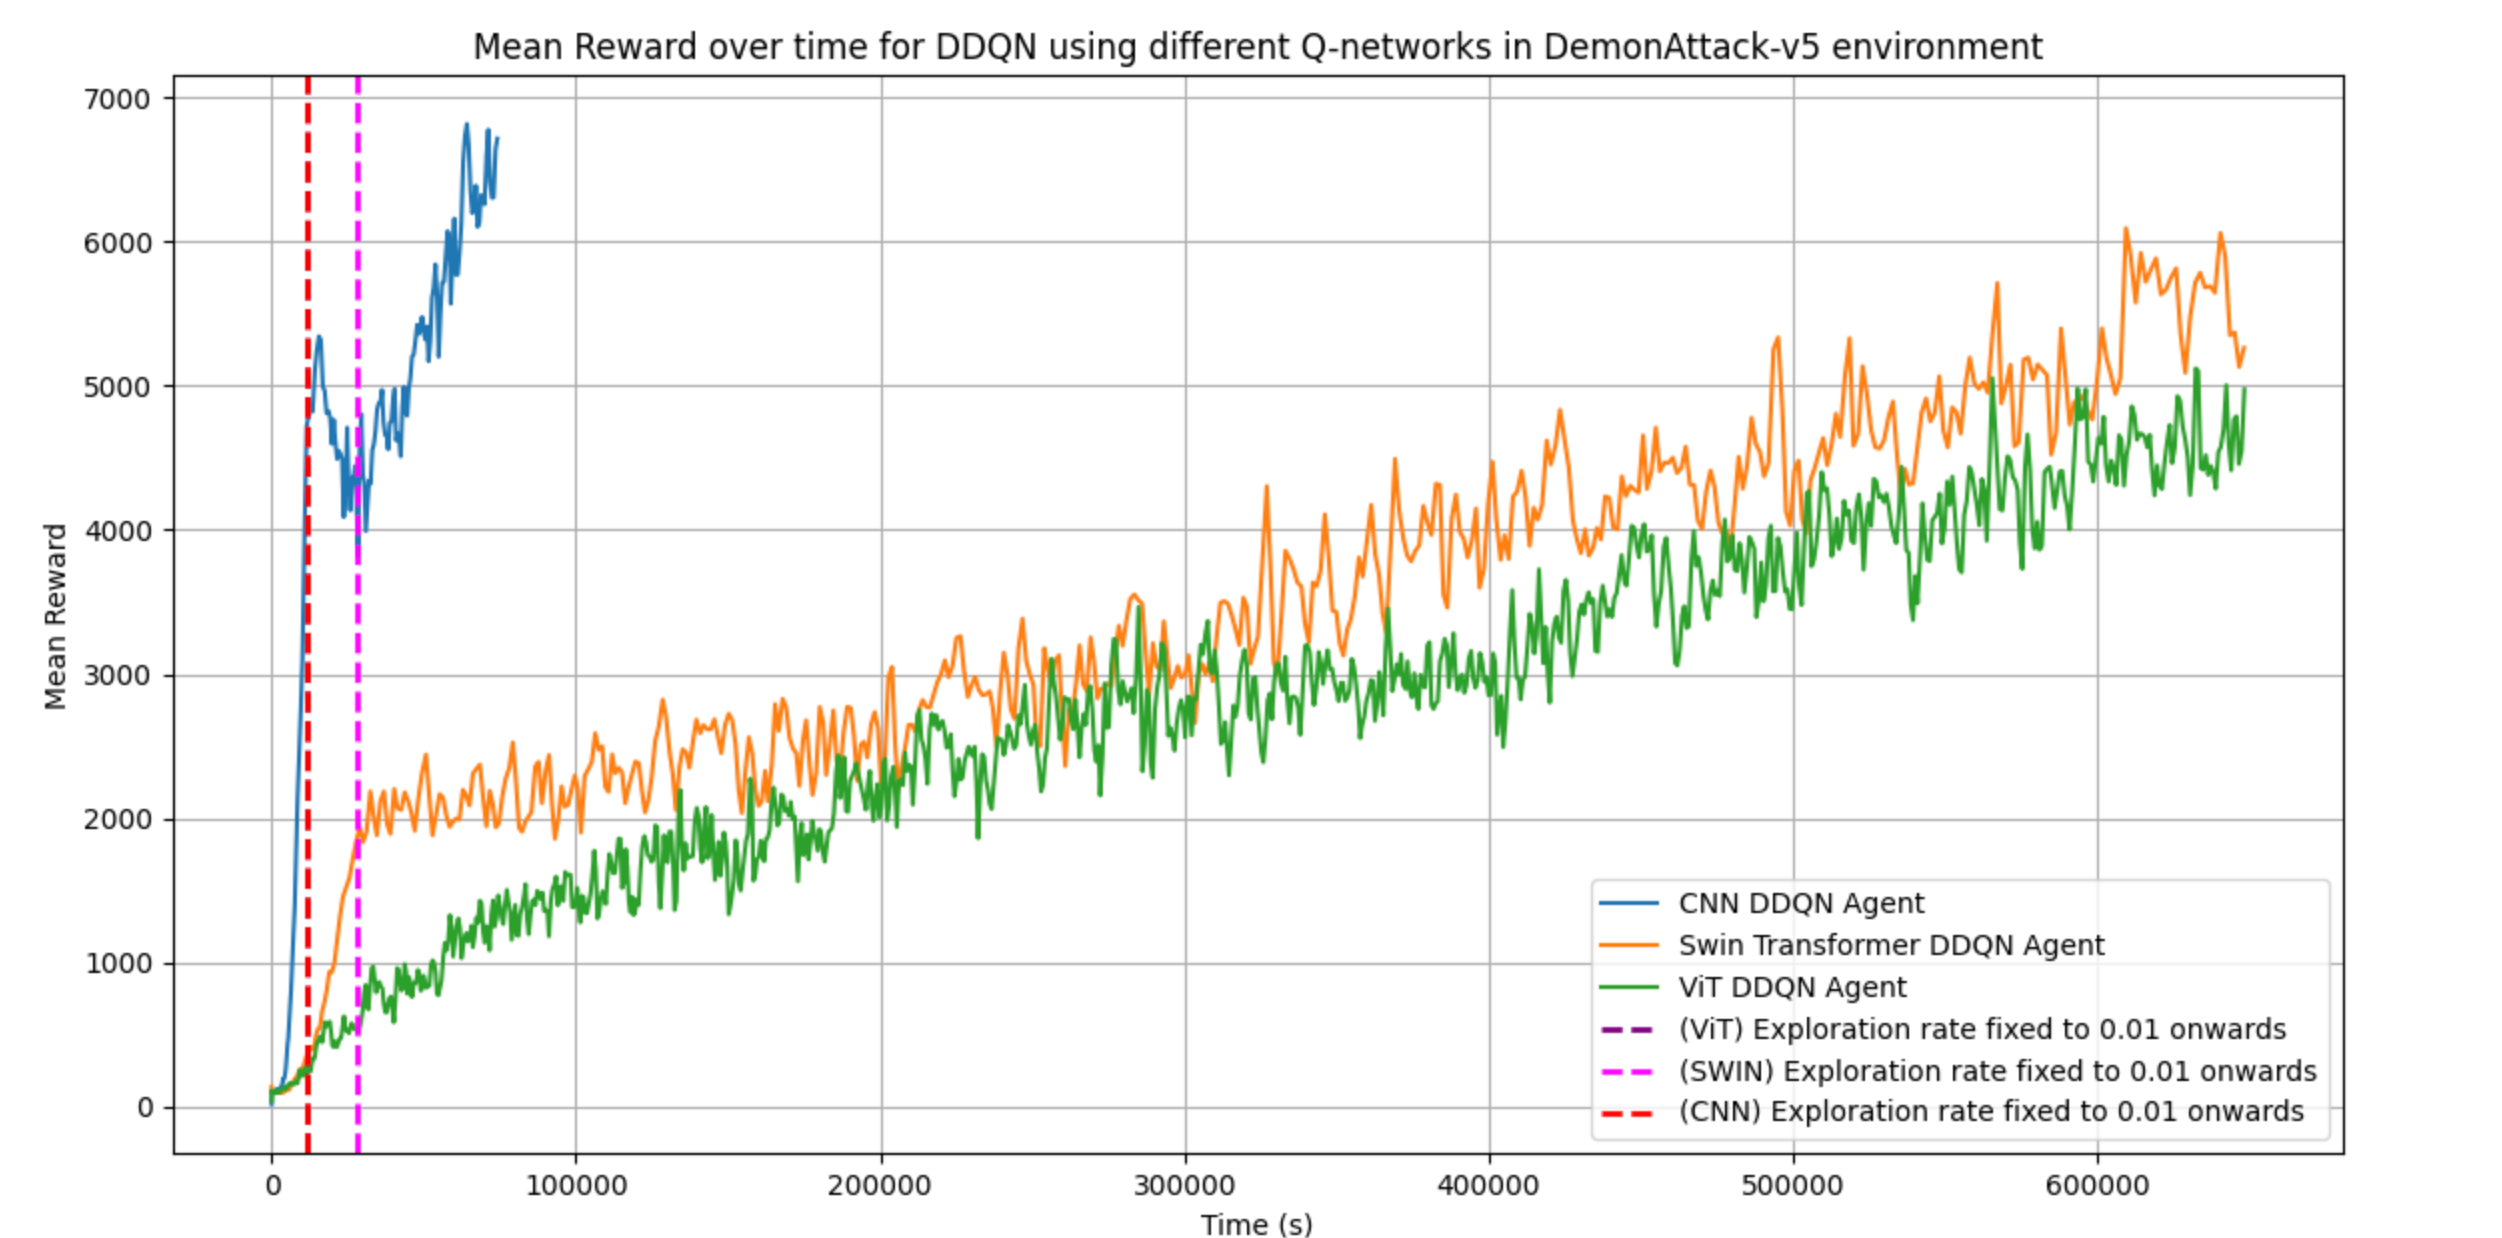
\includegraphics[width=\linewidth]{figures/demon_attack_results_seconds}
	\caption{DemonAttack environment results in seconds.}
	\label{fig:demonattackresultsseconds}
\end{figure}

Finally, in table \ref{tab:demonattack_trainingresults} we summarize the results for the training procedure for the agents. The conditions are the same as in section \ref{sec:mspacman-training-results}, where the exploration rate is fixed to $\epsilon = 0.01$. This table portrays what we have already discussed, as the CNN agent out-performs the attention-based models, especially the ViT, by a considerable margin.

\begin{table}[!h]
	\begin{center}
		\caption[MsPacman environment results for the several trained agents]{DemonAttack environment results for the several trained agents}
		\label{tab:demonattack_trainingresults}
		\begin{tabular}{||c c c c | c||} 
			\hline
			Agent type & Total Time (s) & Total Steps & Total Episodes & Max. Reward \\ [0.5ex] 
			\hline\hline
			CNN & 2 days 1 hours& 6.096 $\times 10^6$ & 10400 &  \textbf{6727}\\ 
			\hline
			SWIN & 7 days 18 hours & 1.936 $\times 10^7$ &  28150 & 6153 \\
			\hline
			ViT & 7 days 18 hours & 3.127 $\times 10^7$ &  51200 & 5120 \\
			\hline
		\end{tabular}
	\end{center}
\end{table}


\subsection{Final evaluation results}
Once the training procedures were done, we proceeded to evaluate the agents in the several environments where we trained them. For this task, we put the agents under "exploit mode", meaning that the exploration rate of the agents was $\epsilon=0$. This differs from how we extracted the results previously explained in sections \ref{sec:mspacman-training-results} and \ref{sec:demon-attack-training-results}, since the maximal scores from the results in training were obtaining with an exploration rate $\epsilon=0.01$. In order to obtain meaningful results, we run, for each environment, each agent for 100 episodes, extracting the mean and the standard deviation from all the runs. The code for extracting these results is in the \href{https://github.com/Javimh18/DL_TFM/blob/main/src/evaluate.py}{evaluate.py} script.

In Table \ref{tab:final_results} we see the final results scores (rewards) for the agents in evaluation mode. For the DemonAttack environment, the CNN agent was the best model. Scores are higher compared to the training results, which makes sense as the agents are completely exploiting the knowledge that they have acquired during the training phase. The SWIN agent actually surprised us, since it closed the gap to the CNN agent by quite a lot. The ViT agent performed the worst achieving a mean score that was less than the half of the CNN agent score. However, in the MsPacman environment things changed quite a lot. The ViT agent was actually the best performing out of the three. Also, it was the most constant in terms of always delivering the same score, since the standard deviation is the smallest of the three of them.

\begin{table}[!h]
	\begin{center}
		\caption[Mean Scores for the trained agents]{Mean Scores for the trained agents}
		\label{tab:final_results}
		\begin{tabular}{||c c c c||} 
			\hline
			Environment& CNN Agent & SWIN agent & ViT agent \\ [0.5ex] 
			\hline\hline
			Demon Attack& \textbf{7865.75 ($\pm$ 2842.26)} & 7741.9 ($\pm$ 2238.2) & 3842.9 ($\pm$ 2208.5) \\ 
			\hline
			Pacman & 5382.3 ($\pm$ 1635.37) & 5829.12 ($\pm$ 2067.05) &  \textbf{6044.71 ($\pm$ 1623.28)} \\
			\hline
		\end{tabular}
	\end{center}
\end{table}

In Table \ref{tab:max_final_results}, the maximum scores for each environment are shown. For the DemonAttack game, the CNN agent was actually the better by quite a margin, consolidating its position as the best performing agent of all them three. In the MsPacman game, something similar occurs for the ViT, as it outperforms by a considerable margin the rest of the agents. Even though the order for the max scores remains the same as the mean scores, in the DemonAttack game, the maximum score is doubled compared to the mean score for the attention-based agent, while it is almost tripled for the CNN agent. On the other hand, this does not happen for the MsPacman game, where the maximum scores are only doubled compared to the mean scores.

\begin{table}[!h]
	\begin{center}
		\caption[Max Scores for the trained agents]{Max Scores for the trained agents}
		\label{tab:max_final_results}
		\begin{tabular}{||c c c c||} 
			\hline
			Environment& CNN Agent & SWIN agent & ViT agent \\ [0.5ex] 
			\hline\hline
			DemonAttack& \textbf{22050} & 14280 & 8415 \\ 
			\hline
			MsPacman & 9330 &  10345 & \textbf{12561} \\
			\hline
		\end{tabular}
	\end{center}
\end{table}

We also took into account the minimum scores of our agents, because we wanted not only to know how good our models can be, but also how bad. For the DemonAttack model, the ViT clinched its position as the worst performer in the game of them all, and by a large margin. In the following sections we will explore the explainability features, and hopefully understand what may happen for this model to not perform as good as we expected. The rest of the scores for both the DemonAttack and MsPacman environments were kind of expected.

\begin{table}[!h]
	\begin{center}
		\caption[Min Scores for the trained agents]{Min Scores for the trained agents}
		\label{tab:min_final_results}
		\begin{tabular}{||c c c c||} 
			\hline
			Environment& CNN Agent & SWIN agent & ViT agent \\ [0.5ex] 
			\hline\hline
			DemonAttack& 1700 & 760 & \textbf{140} \\ 
			\hline
			MsPacman & \textbf{1520} &  1990 & 1940 \\
			\hline
		\end{tabular}
	\end{center}
\end{table}

Additionally, we compared our results with \cite{meng2024deep}, to see how "good" our models were. This comparison made sense for us since, to the best of our knowledge, is the work with the best scores that uses a transformer-based Q-network in the DDQN set-up, called SWIN DQN. They provide results for the whole ALE games, but, since we could only train our agents for two environments, those will be the ones we will comparing ourselves with them. In Table \ref{tab:sota_mean_final_results} we see the mean evaluation results, where in the DemonAttack environment, they outperform our models by almost 12 times. Nevertheless, for the MsPacman game, our ViT agent outperforms their proposed model, achieving a best mean score of over a 100 points.

\begin{table}[!h]
	\begin{center}
		\caption[Comparison with SWIN DQN \cite{meng2024deep} for mean scores for the trained agents]{Comparison with SWIN DQN \cite{meng2024deep} for mean scores for the trained agents}
		\label{tab:sota_mean_final_results}
		\begin{tabular}{||c c c c c||} 
			\hline
			Environment& CNN Agent (ours)& SWIN agent (ours) & ViT agent (ours) & SWIN DQN\\ [0.5ex] 
			\hline\hline
			DemonAttack& 7865.7 ($\pm$ 2842.2) & 7741.9 ($\pm$ 2238.2) & 3842.9 ($\pm$ 2208.5) & \textbf{89254 ($\pm$ 49893)}\\ 
			\hline
			MsPacman & 5382.3 ($\pm$ 1635.3) & 5829.1 ($\pm$ 2067.5) & \textbf{6044.7 ($\pm$ 1623.2)}  & 5878.0 $\pm$ 2426.4 \\
			\hline
		\end{tabular}
	\end{center}
\end{table}

We also compared our agent's performance in terms of maximal scores, where we got beaten by the SWIN DQN agent in both games. In the DemonAttack game, we got beaten by a score that was 5 times better than ours. In the MsPacman environment, we got beaten by over a 1.400 points, even though our mean scores were better. One explanation that we have for this, is that their agent has a larger standard deviation, which means that the agent is less consistent to recurrently obtain similar scores to the mean, for worse, and for better.

\begin{table}[!h]
	\begin{center}
		\caption[Comparison with SWIN DQN \cite{meng2024deep} for max scores for the trained agents]{Comparison with SWIN DQN \cite{meng2024deep} for max scores for the trained agents}
		\label{tab:sota_max_final_results}
		\begin{tabular}{||c c c c c||} 
			\hline
			Environment& CNN Agent (ours) & SWIN agent (ours) & ViT agent (ours) & SWIN DQN  \\ [0.5ex] 
			\hline\hline
			DemonAttack& 22050 & 14280 & 8415 & \textbf{134465}\\ 
			\hline
			MsPacman & 9330 &  10345 & 12561 & \textbf{13911}  \\
			\hline
		\end{tabular}
	\end{center}
\end{table}

\section{Explainability features}
\label{sec:eval_feat_explainability}

\subsection{Attention maps results}
\label{sec:eval_attn_maps_explainability}
For the attention maps, we extracted a whole display of graphs with the aim of providing an insightful analysis on the attention heads for the ViT. Recalling section \ref{sec:extracting_exp_feat}, we remind the reader we could only extract the attention maps for the ViT Q-network

\subsubsection{MsPacman attention maps analysis}
For the MsPacman environment, the extracted maps are displayed in Figure \ref{fig:wholeattnmaps}, where as the colour-bar suggests, the more yellow a section is, the more attention the ViT is paying to it. All the figures presented in this section are part of a set of videos that we have recorded in order to better analyse the sequences when actions are performed. 

\begin{figure}[!h]
	\centering
	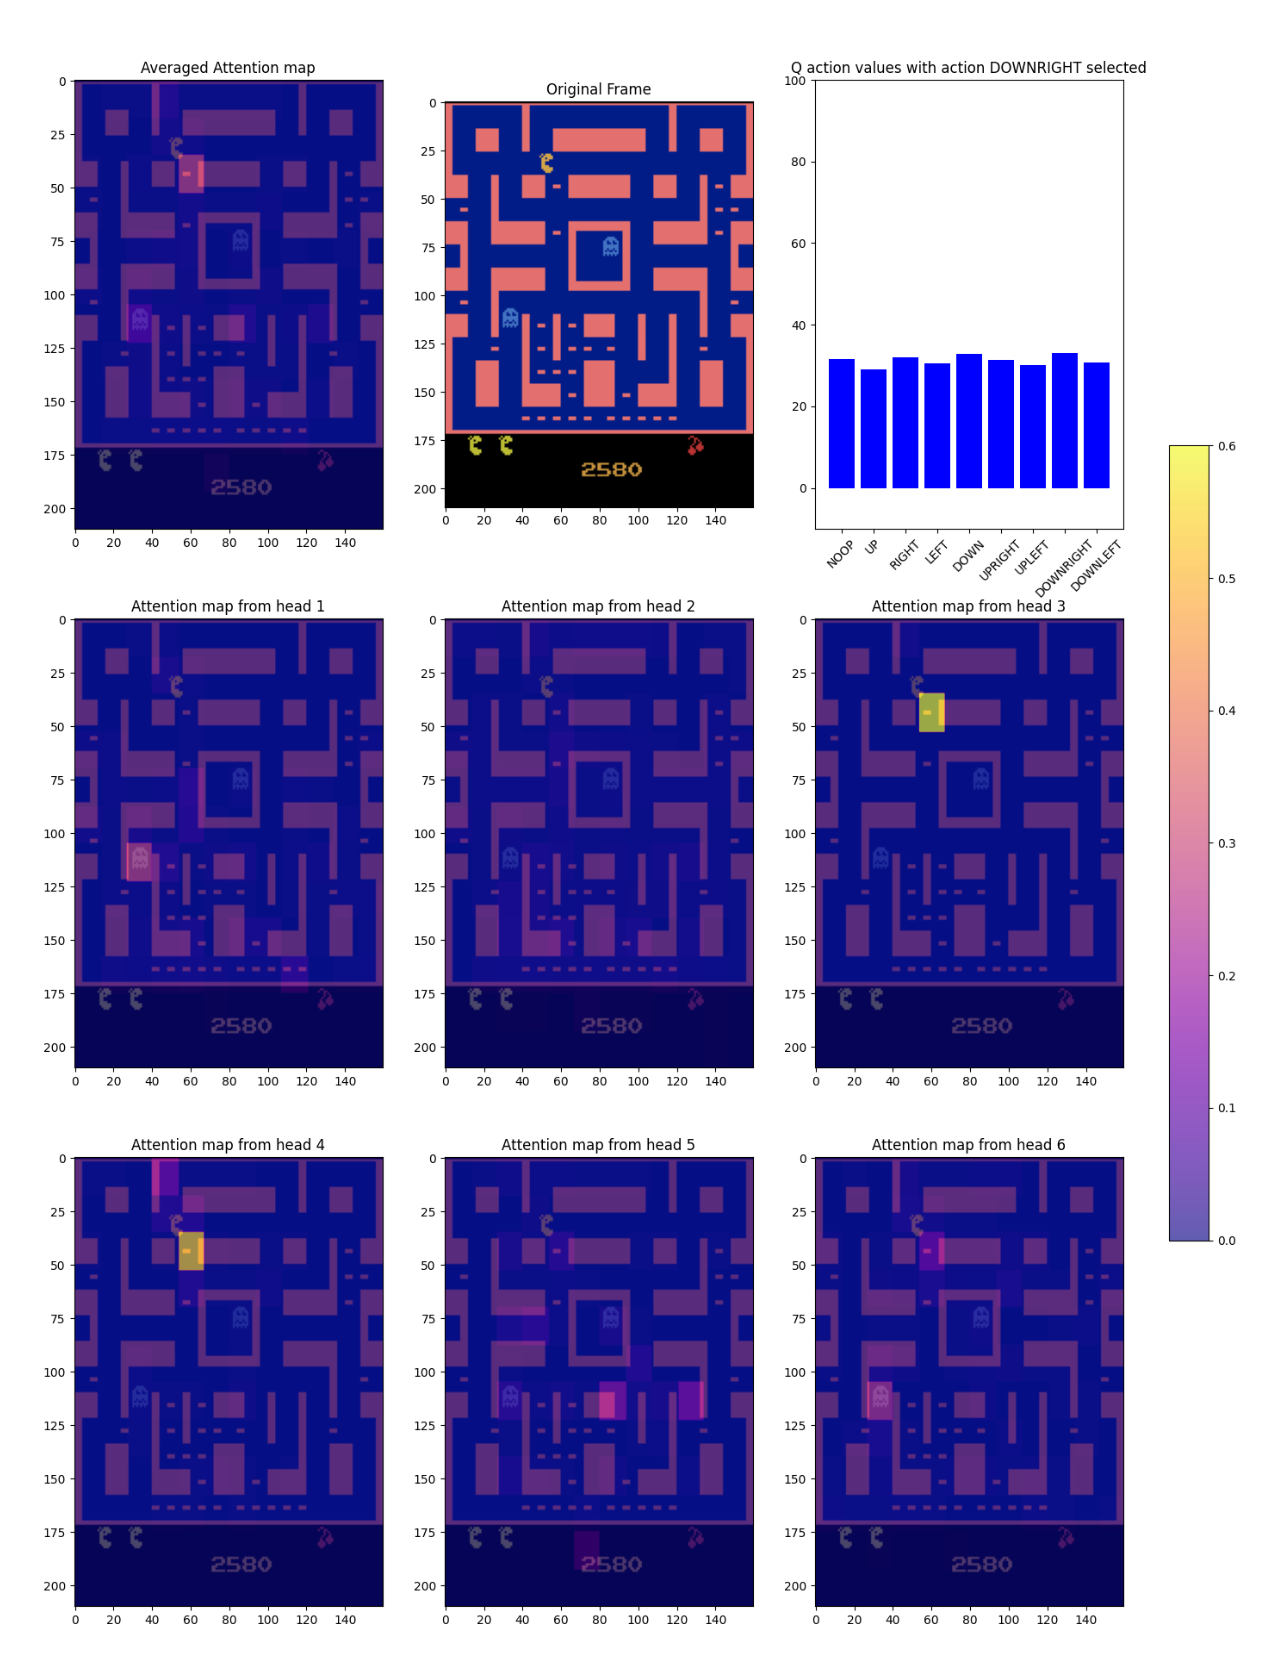
\includegraphics[width=0.75\linewidth]{figures/whole_attn_map}
	\caption{In game frame where we provide (from left to right) the averaged attention map, the original frame and the Q-values as the output of the network. Additionally we provide the attention heads from the ViT Q-network.}
	\label{fig:wholeattnmaps}
\end{figure}

The videos are available in \href{https://drive.google.com/drive/folders/1cABvE9vmXMyWWHmAqBzeffJOcFBc7GZD?usp=sharing}{this} folder in Google Drive. We will try to illustrate as good as we can what we have seen in the videos, but we encourage the readers to see them for themselves, since they provide better context on what we will explain in the following sections. For a better visualization, we used the video player built in Visual Studio Code, since it allows for different reproduction speeds, as does the built-in player in Google Drive.

In general terms, the attention heads pay a lot of attention to where Pacman is in the map, which make a lot of sense, since us humans would actually do the same in order to perform the actions accordingly. But as it can be seen, in Figure \ref{fig:wholeattnmaps}, it additionally pays attention to additional elements in the map, which makes sense also, as we humans can perceive several things at the same time and take into account several factors to perform decision-making.

One of the most critical situations the agent can face in the game is when Pacman encounters a ghost, since it is its principal threat when trying to survive in the game. For example, in Figure \ref{fig:avoidingghosts} we have a series of frames where Pacman encounters a ghost. From left to right, in the first frame, we see an activation in the attention head number 4, acknowledging that the ghost is near Pacman. As frames go by, the attention head number 3 seems to be looking for a place in the map that is safe for Pacman to be, as attention head number 4 intensifies the attention paid to the ghost, that is coming towards Pacman. In the final frame, we actually see how the agent has placed Pacman exactly in the spot it searched frames before.

\begin{figure}[!h]
	\centering
	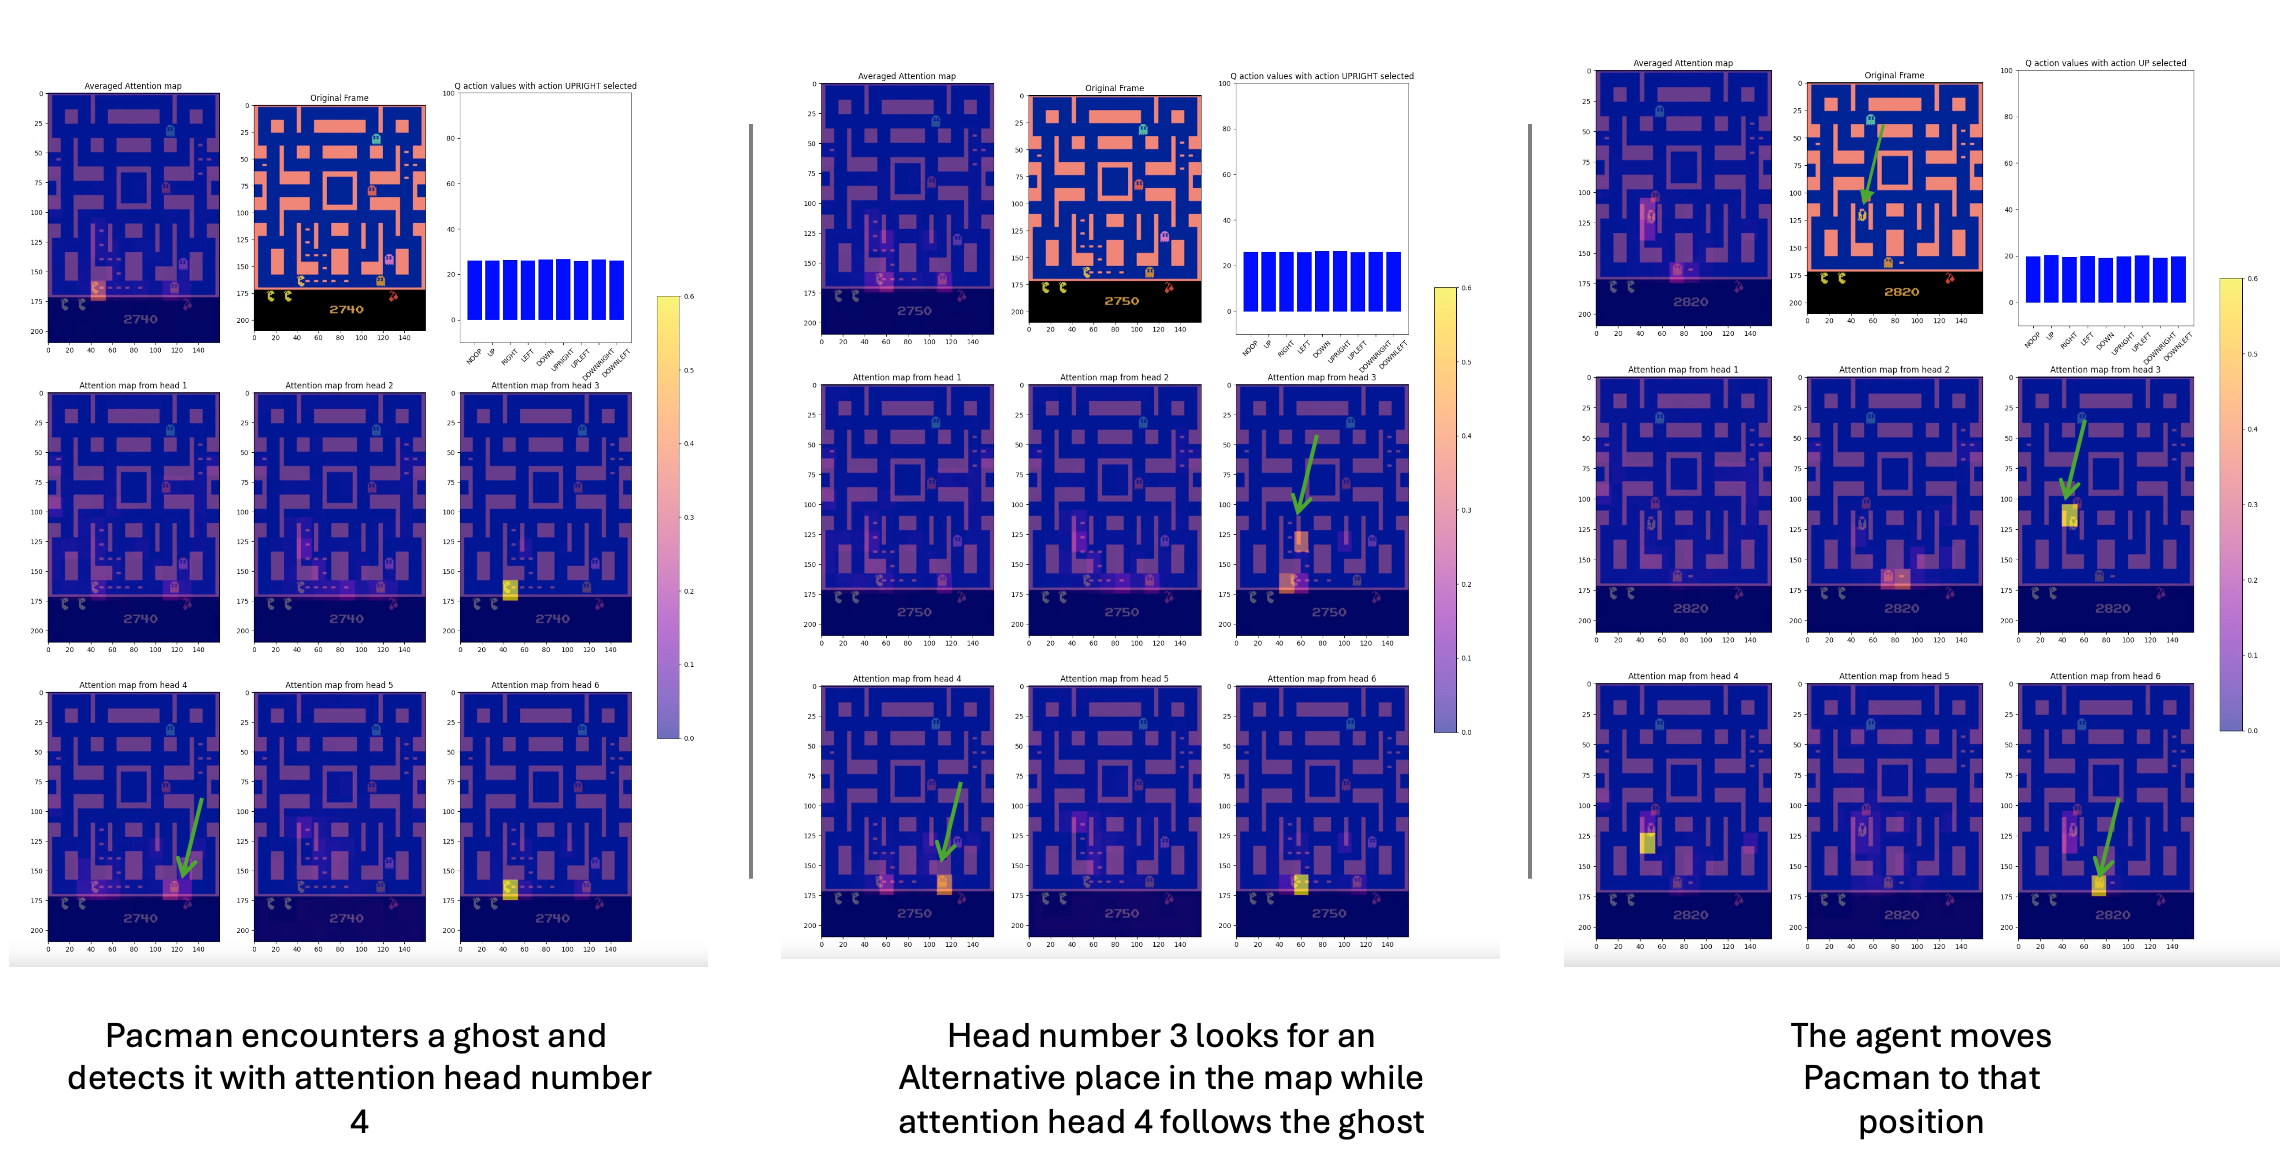
\includegraphics[width=\linewidth]{figures/avoiding_ghost}
	\caption{Three snapshots from a situation where the agent encounters a ghost. It acknowledges the ghost and searches for routes to avoid them.}
	\label{fig:avoidingghosts}
\end{figure}


Extending this phenomenon, we see that the ViT agent attention indicates where it may want to go in the next consecutive frames. In Figure \ref{fig:predictiveattention} we see an example of this. From left to right, in the first frame we see that Pacman is located by the agent in attention head number 4, but attention head number 3 attends to a region of the map which may be of interest. Additionally, attention head number 2 looks for another region of interest (where the tiles are), since there may be potential reward. In the second frame, we see that the agent is going exactly where the attention head 3 payed attention to in the previous image, and that attention head number 2 still paying attention to the section on the map where the tiles are. In the third image, we see that the agent puts Pacman in the section that the attention head 2 was paying attention from the beginning. As we can see, this could be proof that by looking at the attention heads of well-trained models we can effectively predict and understand which are the model's decisions when playing these games and predict which will the next moves or what are the regions of interest for the agent. We remark this phenomenon as it actually happens a frequently in the videos provided in Google Drive.

\begin{figure}[!h]
	\centering
	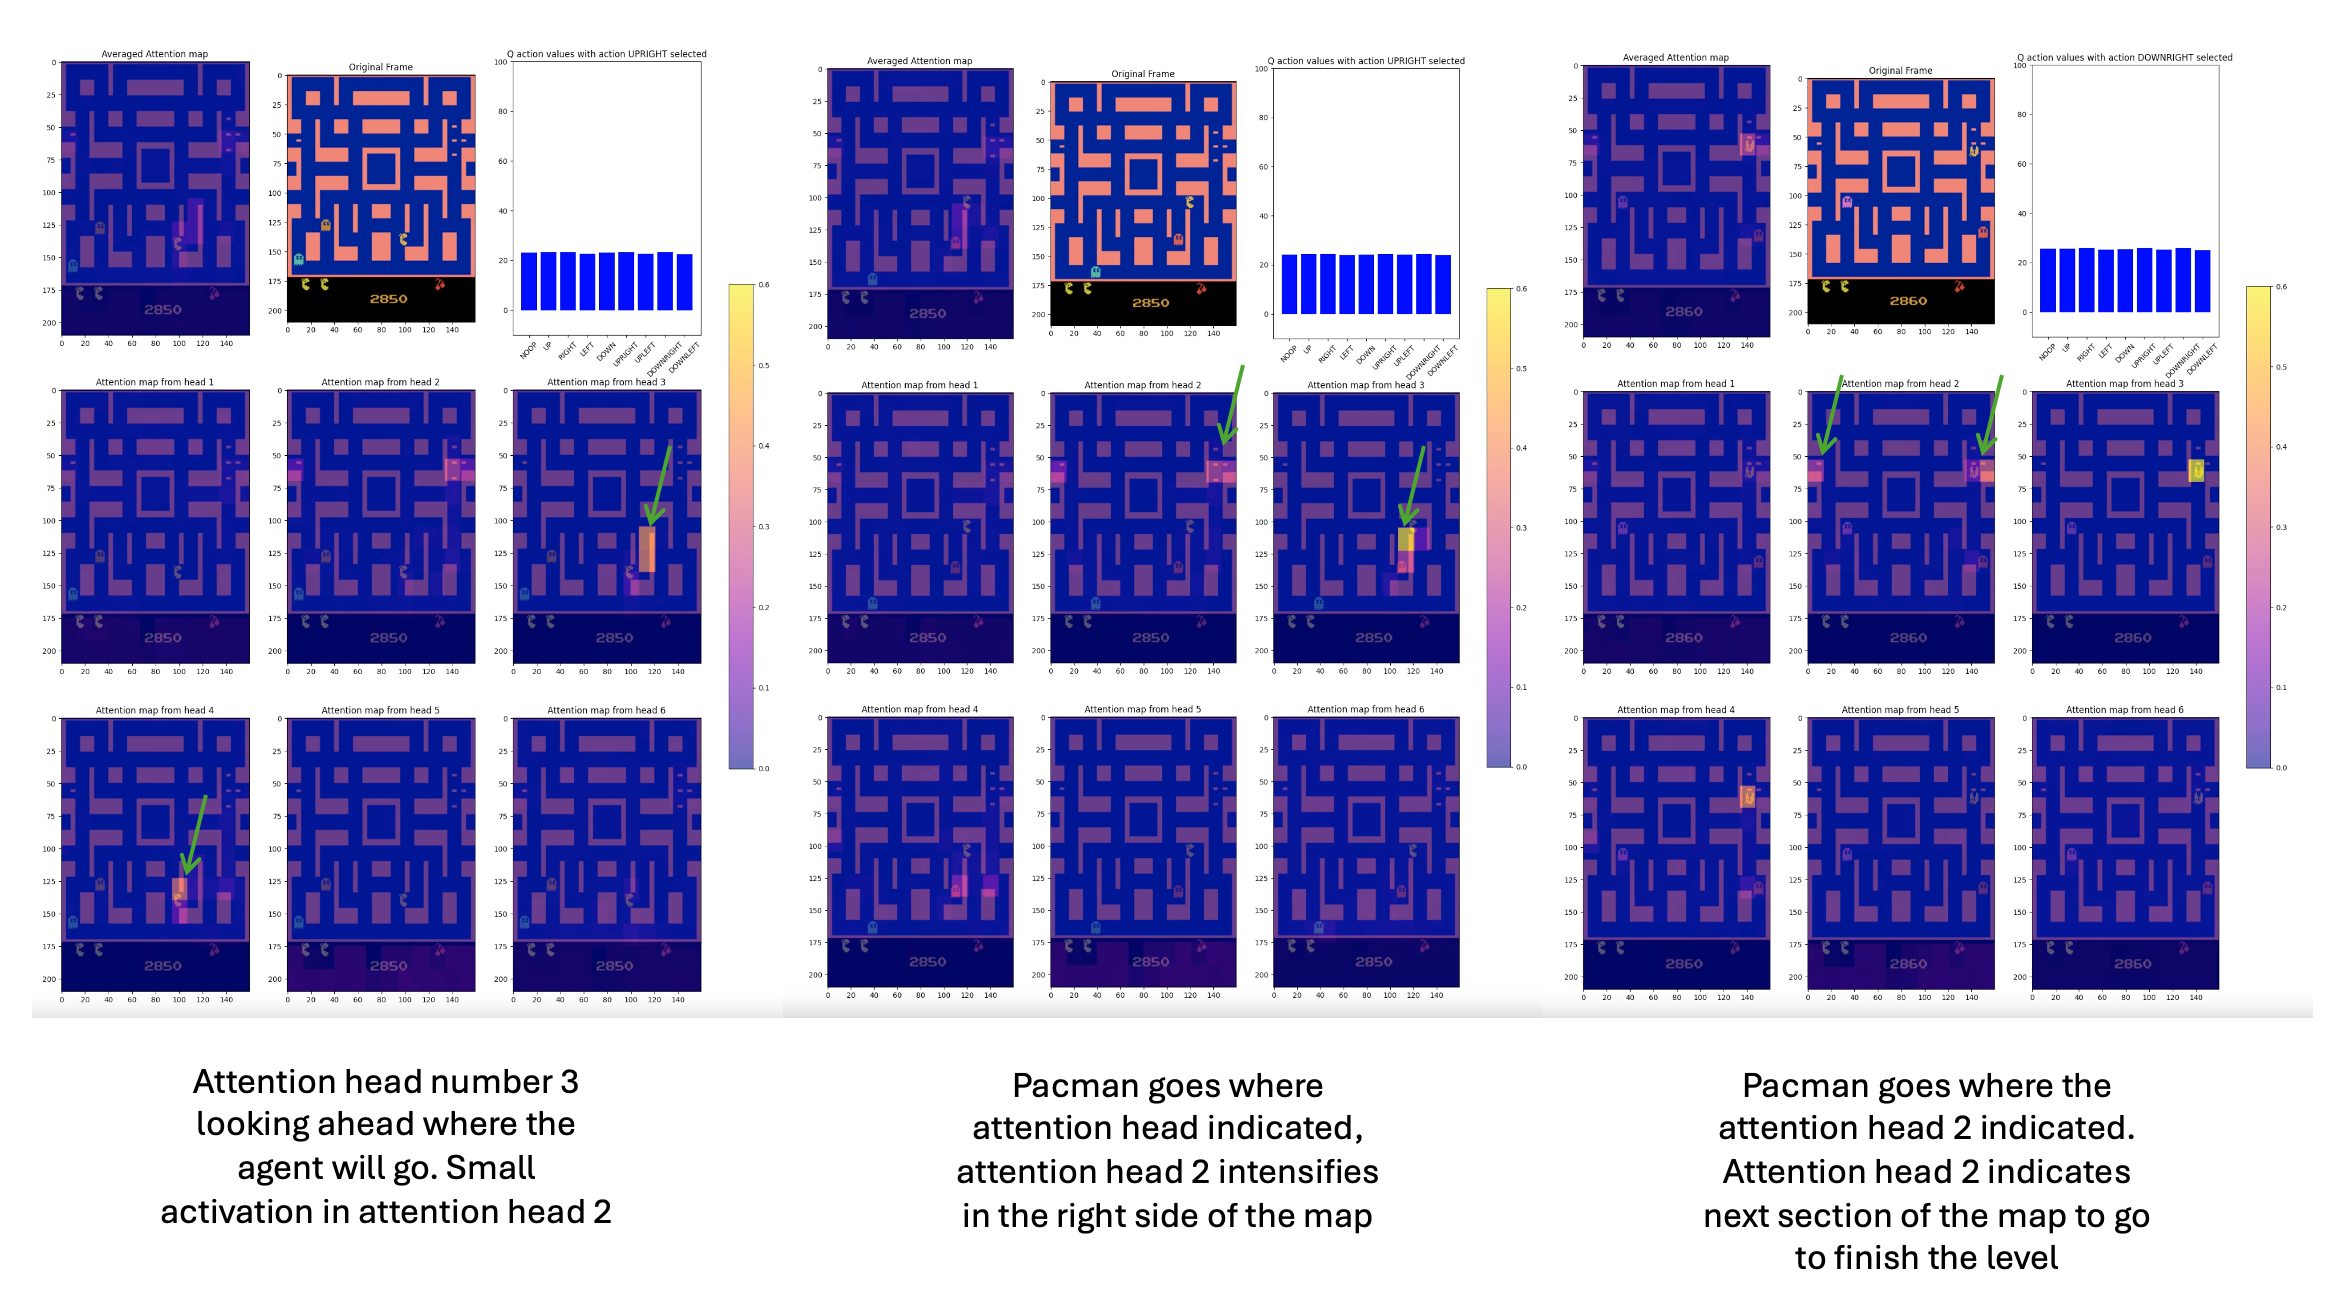
\includegraphics[width=\linewidth]{figures/predictive_attention}
	\caption{Three snapshots from a situation where the agent tries to find rewards in the environment.}
	\label{fig:predictiveattention}
\end{figure}

\subsubsection{DemonAttack attention maps analysis}
For the Demon Attack environment, we collected a series of episodes where we let the agent play, following the same set-up as the previous section. We were aware of the fact that the attention maps from the agent in this environment would not be as interpretable, since the performance from this model was inferior comparatively. Either way, in Figure \ref{fig:demonattackattnmaps} we see a screenshot of the map, where we see the different attention heads. The activations are clearly not as rich as they are in the MsPacman environment. The attention heads pay attention to the shooter, since its the most important part of the game, but it lacks on amplifying the context. For example, attention heads 1 and 5 do not give any important information, and the activations are 0 for almost the entire part of the game. These heads should be adding information, giving a richer and broader context of the state, so that the Q-network provides accurate estimations on the Q-values for the actions. There is a phenomenon that is even worse, as the attention heads 3 and 6 are paying attention to useless sections of the map, like the bottom part, where there is not relevant information for the gamer to actually obtain greater rewards. In figure \ref{fig:demonattackattnmaps2}, we saw that, as the game progresses, the agent starts to pay attention to the scoreboard. We actually think this is a shortcut \cite{Geirhos2020} from the Q-network, since no real reward is obtained by looking directly at the scoreboard, but it might learn in some stage of the game that in that section something interesting usually happens (maybe because the enemies usually appear from the top section of the game). We felt discouraged by the performance of this agent, because it was the best in the MsPacman game, but then we also realized that attention maps explain the poor behaviour of the model, as it is giving us hints on why it does not perform well. This can be useful when comparing different models based on attention, as we have seen that they will effectively describe what is the model looking for in order to perform decision-making. With respect to the agent's performance, as we are writing this, we are trying to improve the model, with the hopes of confirming what we have stated in previous sections, and remains as future work in this line of research.

\begin{figure}[htbp]
	\centering
	\begin{subfigure}{0.48\textwidth}
		\centering
		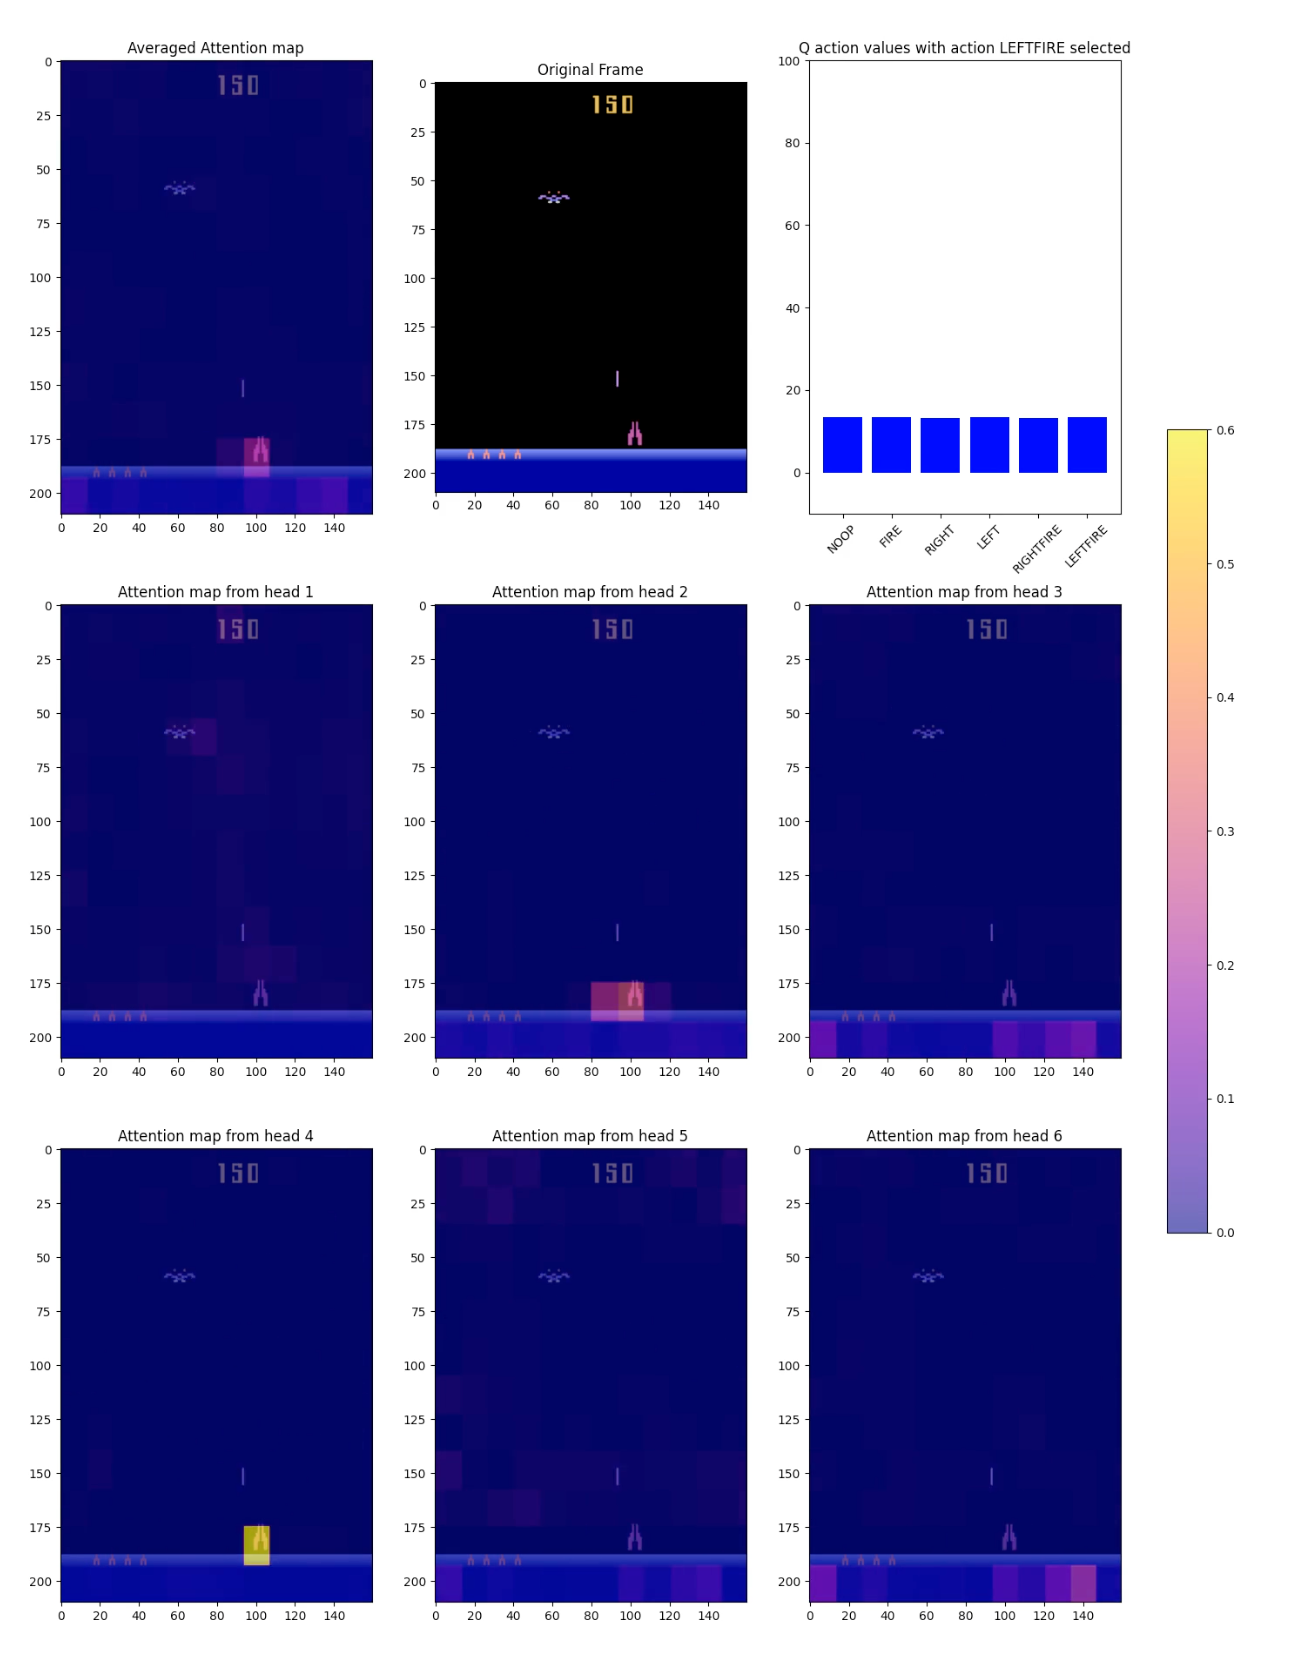
\includegraphics[width=\linewidth]{figures/demonattack_attn_maps}
		\caption{}
		\label{fig:demonattackattnmaps}
	\end{subfigure}
	\begin{subfigure}{0.48\textwidth}
		\centering
		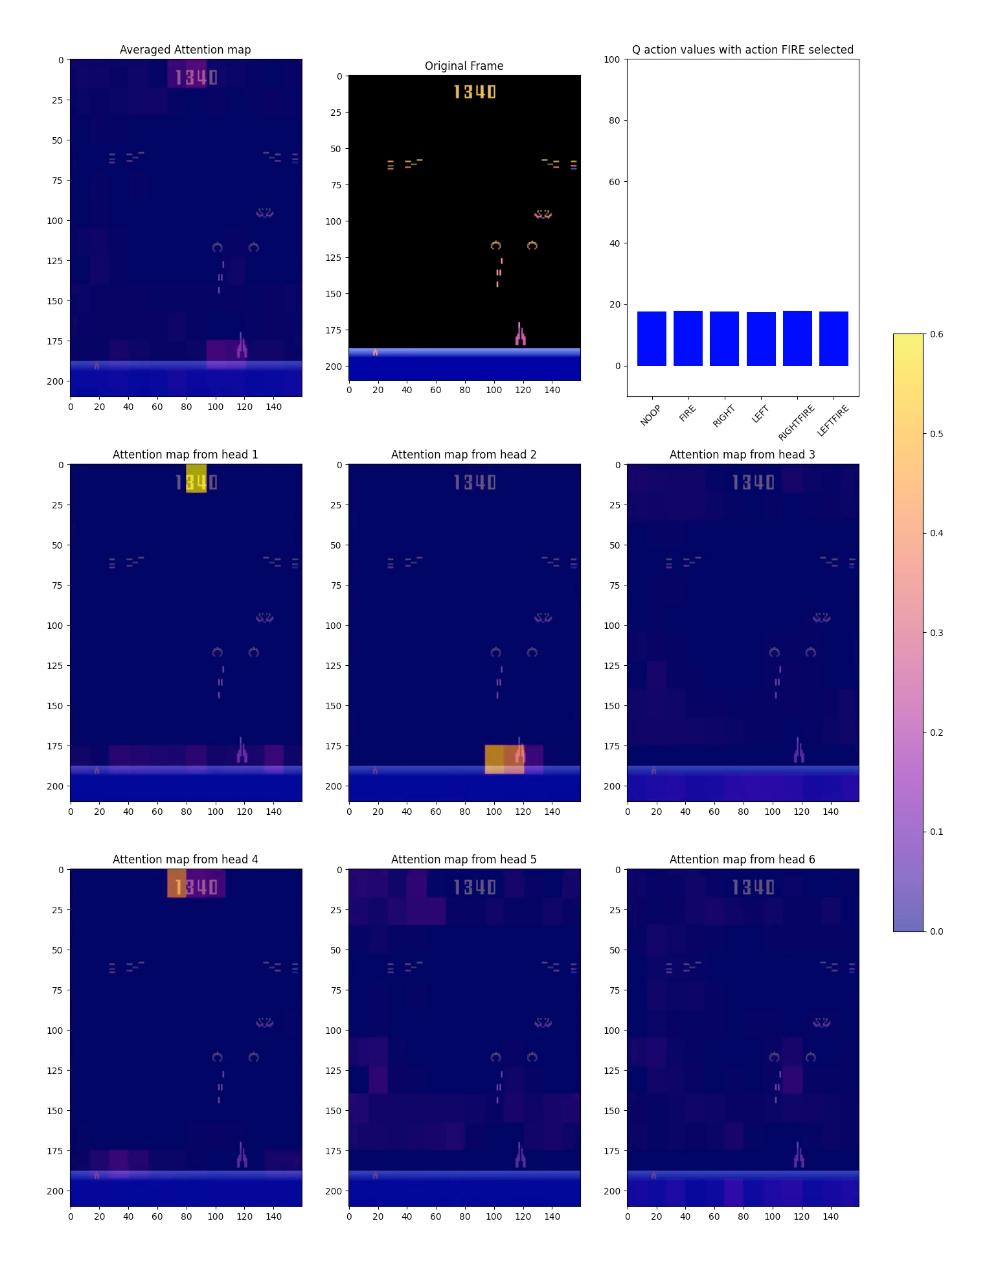
\includegraphics[width=\linewidth]{figures/demonattack_attn_maps2}
		\caption{}
		\label{fig:demonattackattnmaps2}
	\end{subfigure}
	\caption{Attention maps for the DemonAttack environment.}
	\label{}
\end{figure}

\subsection{Activation maps results}
\label{sec:eval_actv_explainability}
Once we analysed the attention maps for the ViT agent, we proceeded to evaluate the activation maps that Grad-CAM provided for both the ViT and the SWIN Transformer agents. We did not evaluate the CNN agent because we wanted to prioritize the attention-based models, as that is the aim of this work. However, we keep this task as future work.

\subsubsection{MsPacman Activation maps analysis}
For the ViT agent, the activations are shown in Figure \ref{fig:vitactivationmapsgradcamframe1}. We show a set of three frames from different stages of the game (as it can be seen by checking the score). It is pretty clear that the ViT agent does only care about one thing, the tiles. From top to bottom, we see that in the first stages of the game, the agent has big activations everywhere, since there are a lot of tiles scattered throughout the maze. As the agent starts to move around, eating lots of the tiles, the activation maps show that the sections of the map where there are still tiles have high activation, while sections where there are no tiles have no activation. This matches a lot with the intuition that we were getting about the agent, since it seemed it mostly cared about eating the tiles.

\begin{figure}[!h]
	\centering
	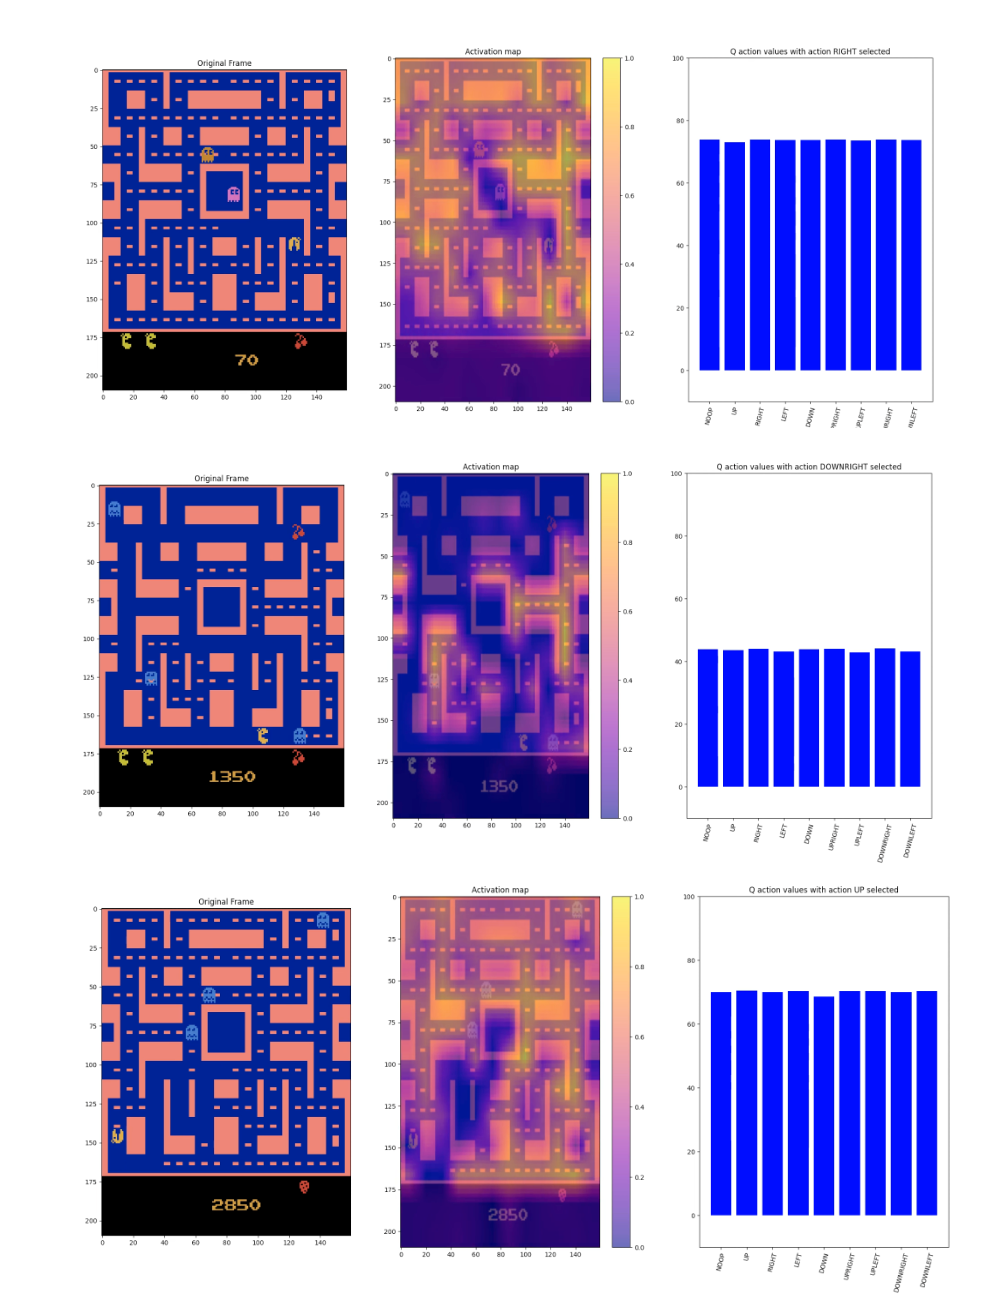
\includegraphics[width=0.7\linewidth]{figures/vit_activation_maps_grad_cam_frame1}
	\caption{Several Grad-CAM activations over different phases of the MsPacman game for the ViT agent.}
	\label{fig:vitactivationmapsgradcamframe1}
\end{figure}

And it seems like the tiles are the logical option for the agent in order to maximize the reward. Recalling equation \ref{eq:state_value}, the value of a state depends on the reward that we obtain not only from the time-step we are in, but also for the potential rewards the agent may land on in future time-steps. Where we are at the beginning of the game, a lot of potential rewards are available, and that is what we think Grad-CAM is showing with these activation maps. As the tiles are eaten, the agent seems to lose those in the sections of the map where there are no tiles. This also matches with the Q-values the agent predicts. When the game starts, lots of potential rewards can be achieved with almost any action, hence in the top section, the Q-values are high for every action. As long as the game progresses, the number of rewards decay, and so does the Q-values for every action. When the ViT agent finds itself again in a position where lots of potential rewards are available (since it has moved-up one level), the Q-values grow again, correlating with the increasing area in the map where the activations are the highest.

For the SWIN transformer, the activation maps were actually far less interpretable. We show in Figure \ref{fig:swinactivationmapsgradcamframe1} a set of frames where the SWIN agent is (hardly) interpretable, since we can see that the higher activations where in sections of interest of the map. The rest of the activation maps were actually non-sense. For example, in figure \ref{fig:swinactivationnonsense}, we see a activation map that does not make sense given the state, and like this, there are lots of them in the evidences that we extracted. We have two hypothesis on why this may not be working. First, there is a compression in the spatial features in the SWIN transformer, in the Patch Merging layer to be concrete. This compression may be altering the features in ways that we cannot comprehend, hence providing this activation maps. The second is that Grad-CAM is supposed to be used in networks that have been trained under classification task, and although there are some similarities between classifying images and select actions for a given state, the truth is that the losses used to train these models differ, since the classification task uses cross entropy loss and DQN uses the MSE.

\begin{figure}[!h]
	\centering
	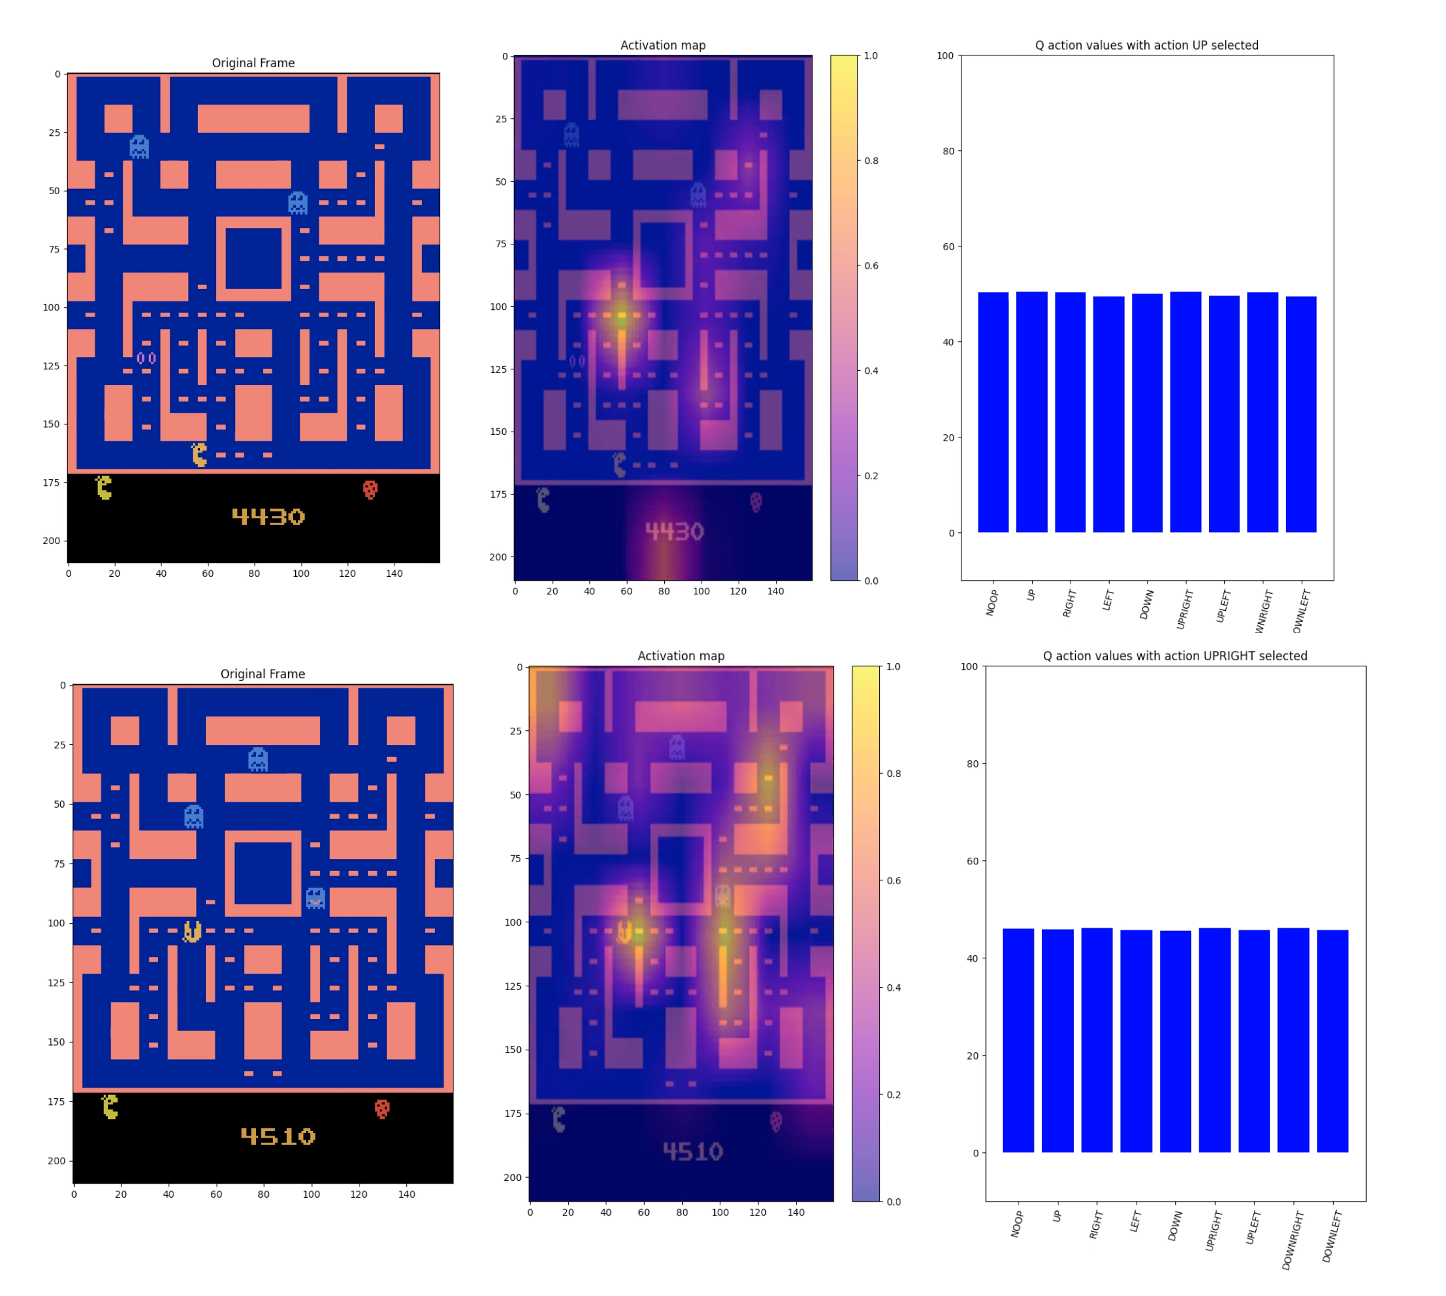
\includegraphics[width=0.65\linewidth]{figures/swin_activation_maps_grad_cam_frame1}
	\caption{Several Grad-CAM activations over different phases of the MsPacman game for the SWIN transformer agent.}
	\label{fig:swinactivationmapsgradcamframe1}
\end{figure}

\begin{figure}[!h]
	\centering
	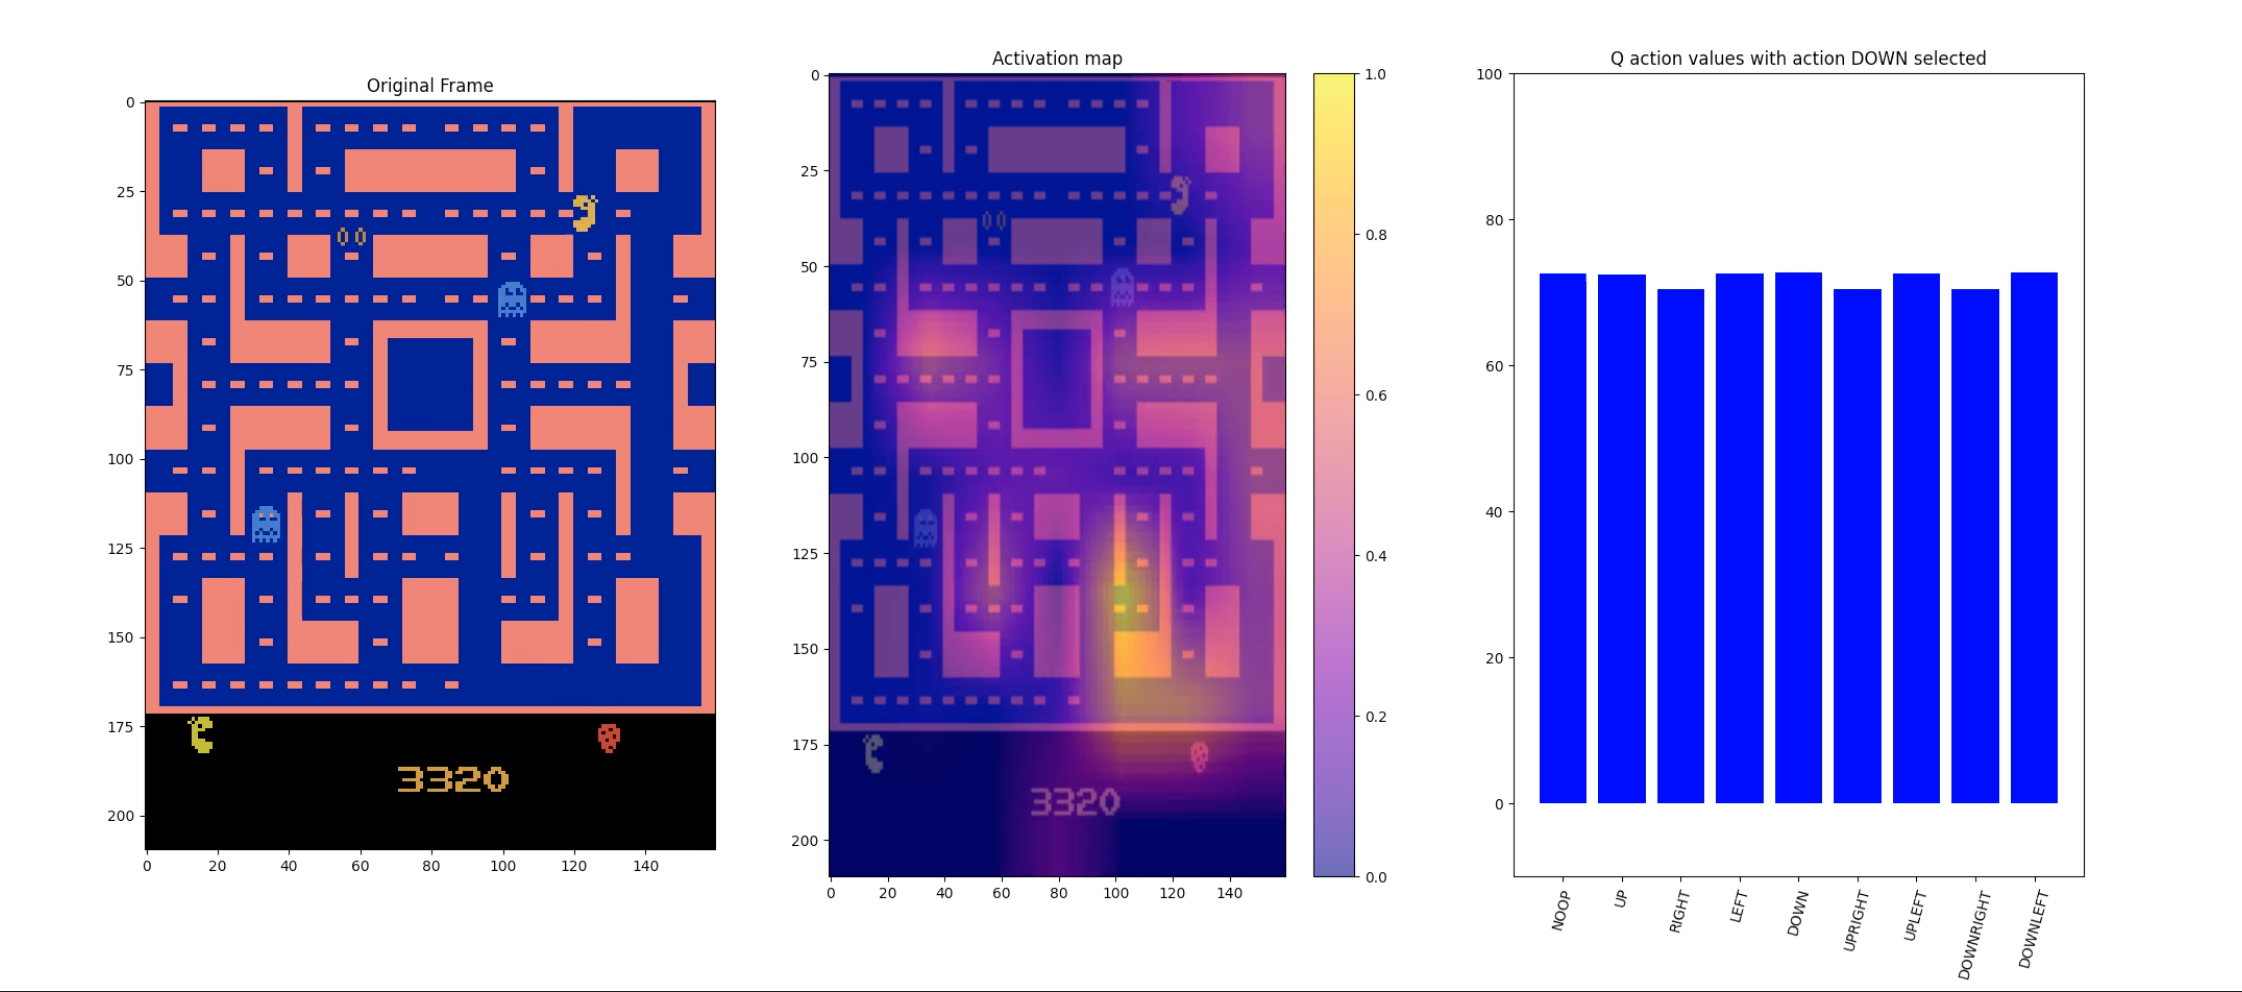
\includegraphics[width=0.65\linewidth]{figures/swin_activation_nonsense}
	\caption{Grad-CAM activations for the MsPacman game for the SWIN transformer agent, where it is clear that it is not understandable what is the agent looking for.}
	\label{fig:swinactivationnonsense}
\end{figure}

\subsubsection{DemonAttack Activation maps analysis}

The activation maps of the ViT agent for the DemonAttack game are available in Figure \ref{fig:demonattackactmapsvit}. From top to bottom, we see that the frame at the top shows no activations whatsoever, with the exception of the score board, which matches with what the attention maps were showing, although we still believe it does not make sense in terms of the context. For the other two activation maps, we see precisely the opposite, as the activations are all around the frame, even at the bottom of the screen, but there are no activations in the scoreboard. Opposite to what we encountered in the MsPacman environment, here, the activation maps seems to not correlate with what is going on in the game or the Q-values that the Q-network is estimating.

\begin{figure}[!h]
	\centering
	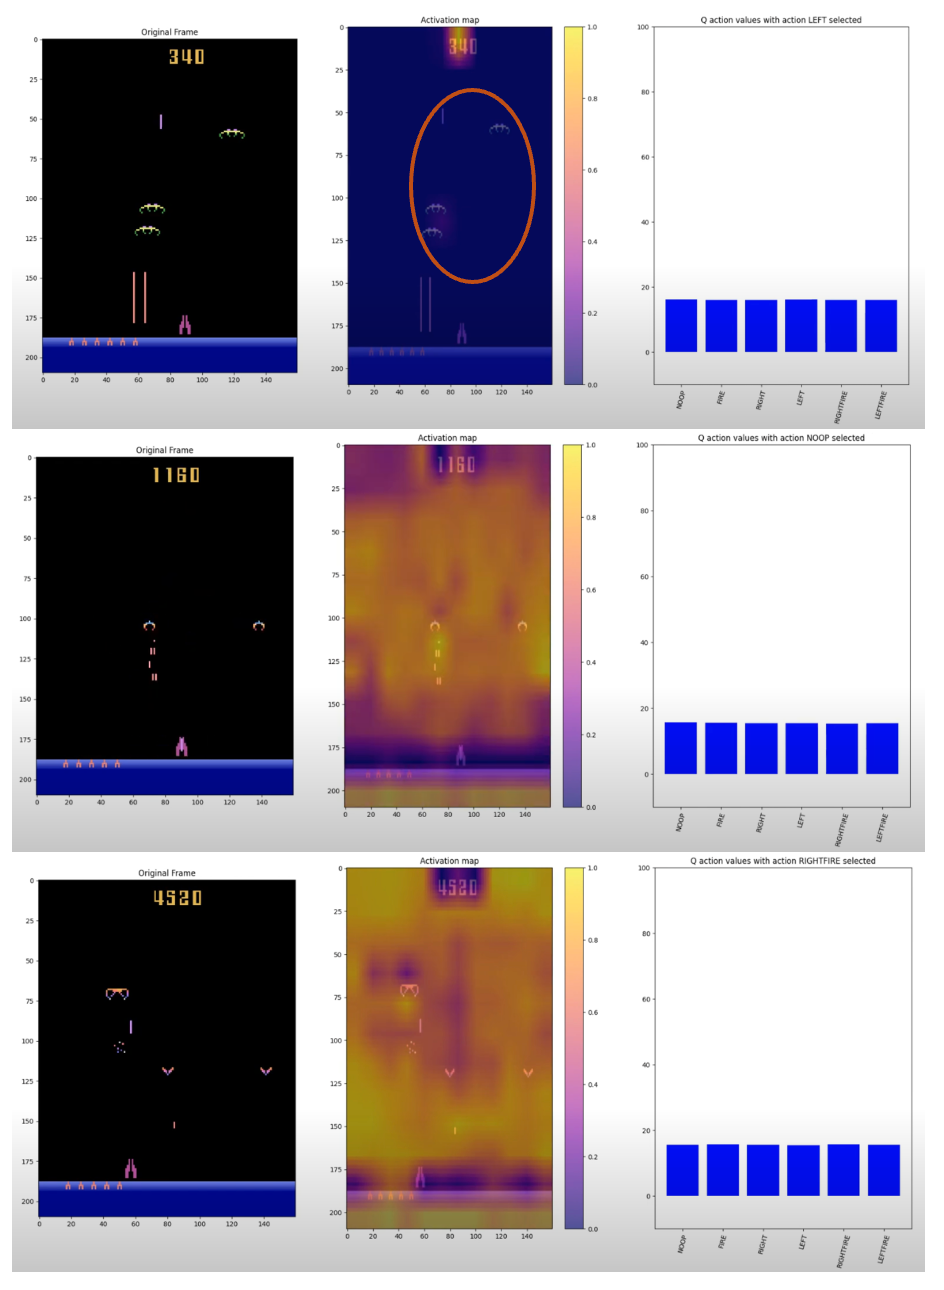
\includegraphics[width=0.7\linewidth]{figures/demonattack_act_maps_vit}
	\caption{}
	\label{fig:demonattackactmapsvit}
\end{figure}

The activation maps of the SWIN agent for the DemonAttack game are available in Figure \ref{fig:demonattackactmaps}. From top to bottom, we see that the frame at the top shows a bit of more understandable activation maps, since they are more interpretable as it usually has greater activations for sections where the enemies are. Nevertheless, the middle and the bottom images show that the activation maps are not quite reliable, since they miss lots of enemies in the frames, as we added some orange circles in the sections where the enemies are present, but no activation seems to appear. This may prove that we are using Grad-CAM in a set-up where we may not be exploiting all its capabilities.

\begin{figure}[!h]
	\centering
	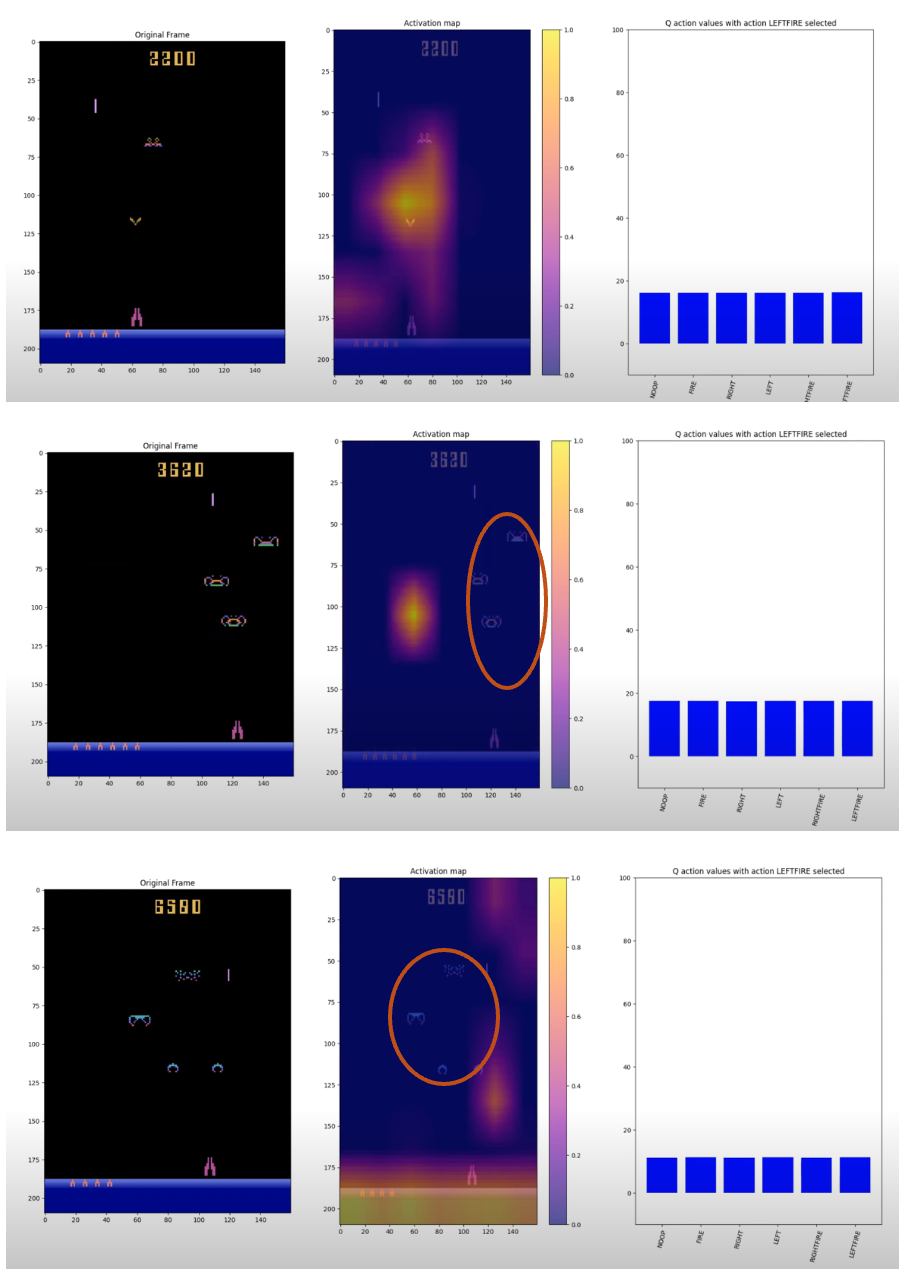
\includegraphics[width=0.7\linewidth]{figures/demonattack_act_maps}
	\caption{Activation maps for the SWIN agent in the Demon Attack environment. Some improvements are obtained in terms of interpretability, but nothing conclusive.}
	\label{fig:demonattackactmaps}
\end{figure}
 
As bottom-line for this section, we can confirm that the Grad-CAM method is not consistent providing explainable or interpretable features so we can understand what is the agent looking for in order to perform in-game decisions.

